One of the key findings of the state of the art chapter \ref{sota}, is the gap that exists in tackling the problem of metamodel and code co-evolution. Most of the existing literature about evolution in Model-Driven Engineering, concerns the artifacts of models, constraints, and transformations, but rarely code. In this chapter, I present my contribution to address the challenge \Circled{\hyperref[C1]{C1}} about resolving the impact of the metamodel evolution on the code automatically. 
This chapter is structured as follows. Section \ref{example} introduces a motivating example showing the breaking impact of the metamodel evolution on the code. 
In section~\ref{approach}, I present the overall automatic co-evolution approach. This approach starts by using the output changes of the metamodel, then it retrieves the errors that are caused by these changes. Thanks to the pattern matching, for each error a resolution is selected and executed. I first give a brief reminder about metamodel changes' detection and why we selected the approach of Khelladi et al.~\cite{khelladi2016detecting}, and how its output is used in the approach. After that, I explain the error retrieval process, followed by a short subsection about the resolution catalog that I use. In the next subsections, I detail the pattern matching phase and the repair mechanism. The overall approach ends with a presentation of the prototype implementation.
Section~\ref{eval} details our evaluation that includes four research questions. These research questions aim to 1) assess the applicability of the approach, 2) to measure its efficiency and its behavioral correctness 3) to compare it with IDE quick fixes as a first baseline, and 4) to compare it with the approach of Khelladi et al.~\cite{Khelladi2020} as a second baseline. This section ends with the evaluation results, followed by threats to validity in Section \ref{ch1_threat}. Finally, Section~ \ref{ch1_conclusion} concludes the chapter with a summary and highlights the approach main contributions. %reflects on future work.
%\begin{wrapfigure}[0.5]{R}{0.5\textwidth}
\begin{figure*}[t]\centering%
	%\scalebox{0.9}{\small\input{pics/diagram-20220513}}%overallApproach}}
	%\vspace*{-0.3cm}
	\centering
	%	\hspace{-0.9cm}
	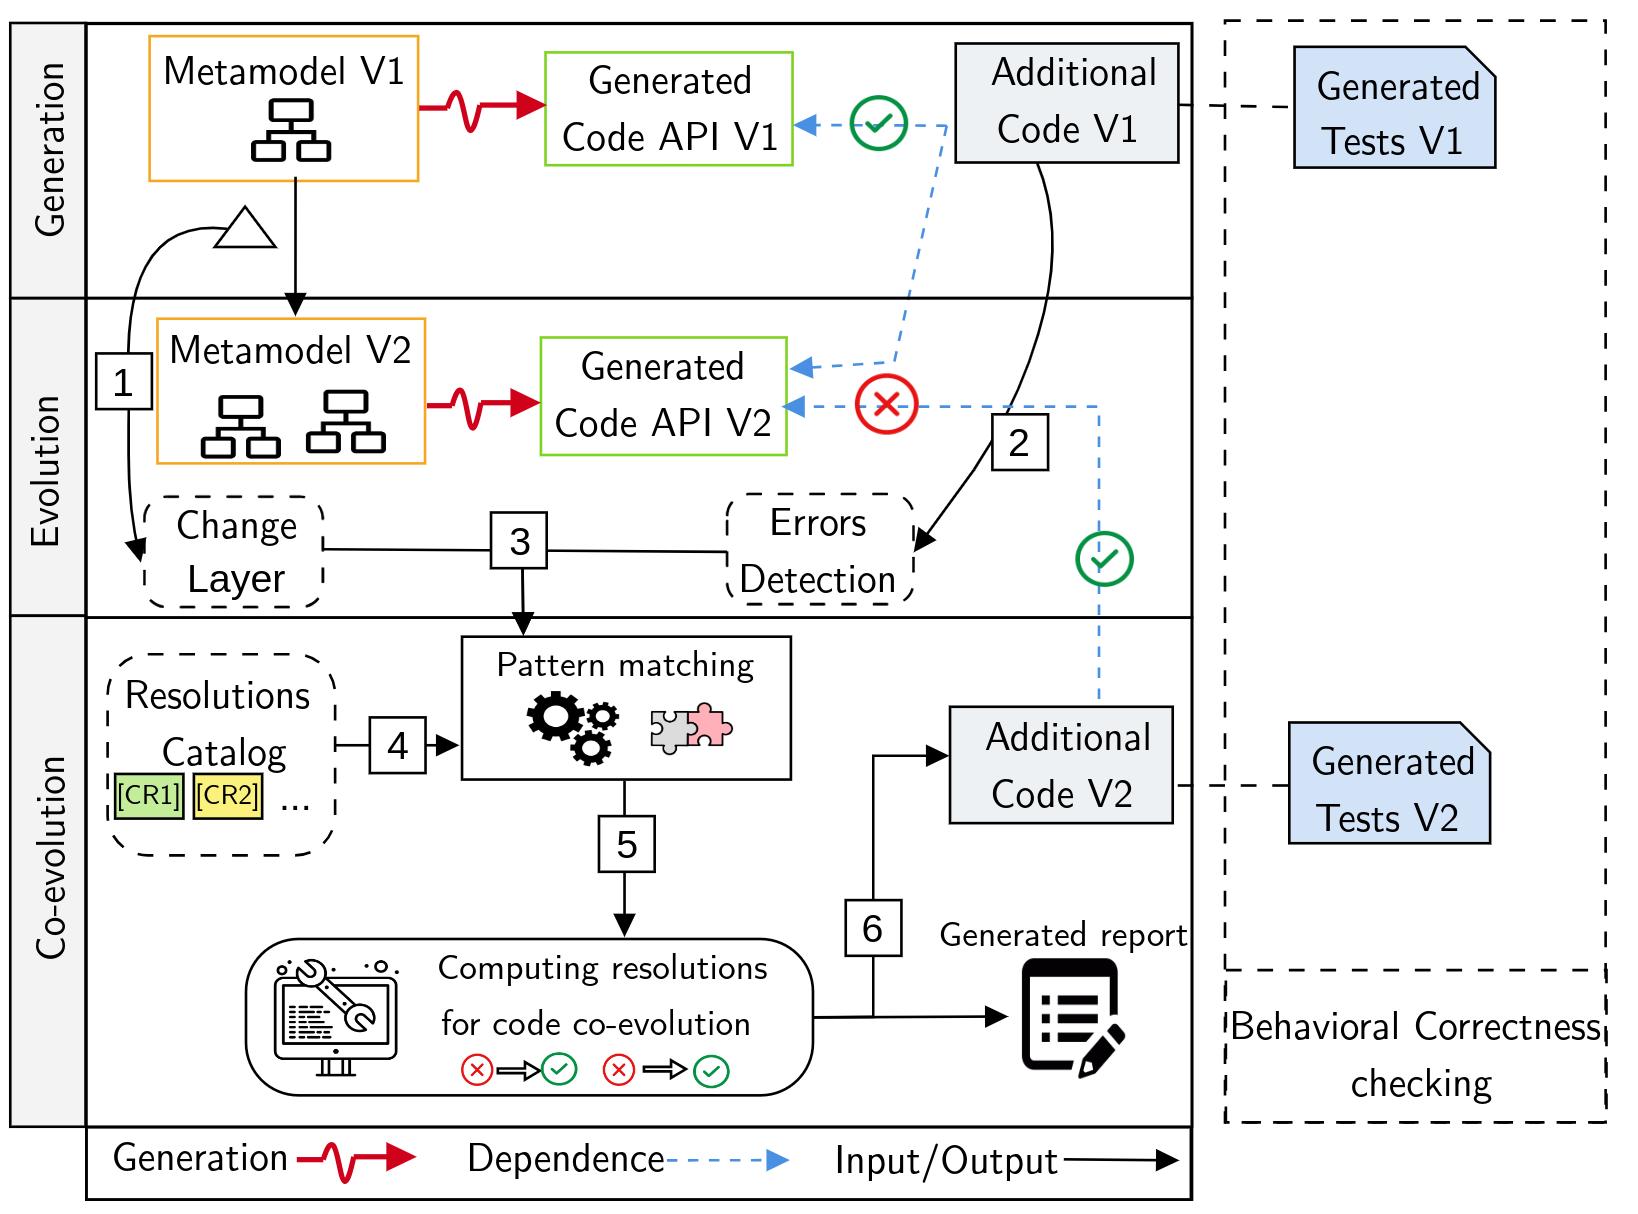
\includegraphics[width=0.8\textwidth]{./pics/chapter1pics/ApproachV5.png}
	\caption{Overall approach for metamodel and code co-evolution}
	\label{fig:overallapproach}
	%\vspace{-1em}
	\vspace{-1em}
\end{figure*}
%\end{wrapfigure}
%\section{Change detection}
\label{sec: ap1_changedetection}

\section{Motivating Example}\label{example}

This section introduces a motivating example to illustrate the challenge of metamodel and code co-evolution. 
Let us take as an example the Modisco project \cite{MDTModisco}, which has evolved numerous times in the past. Modisco is an academic initiative project implemented in the Eclipse platform to support the development of model-driven tools, reverse engineering, verification, and transformation of existing software systems \cite{bruneliere2010modisco,bruneliere2014modisco}.


Figure \ref{fig: BMM} shows an excerpt of the "Modisco Discovery Benchmark" metamodel\footnote{\url{https://git.eclipse.org/r/plugins/gitiles/modisco/org.eclipse.modisco/+/refs/tags/0.12.1/org.eclipse.modisco.infra.discovery.benchmark/model/benchmark.ecore}} consisting of 10 classes in version~0.9.0.
It illustrates some of the domain concepts \textbf{Discovery}, \textbf{Project}, and \textbf{ProjectDiscovery}  used for the discovery and reverse engineering of an existing software system. 
From these metaclasses, a first code API is generated, containing Java interfaces and their implementation classes, a factory, a package, etc. Listing \ref{lis:Modisco_Code_API_V1} shows a snippet of the generated Java interfaces and classes from the metamodel in Figure \ref{fig: BMM}. 

The generated code API is further enriched by the developers with additional code functionalities in the "Modisco Discovery Benchmark" project and its dependent projects as well.
For instance, by implementing the methods defined in metaclasses and advanced functionalities in new classes. Listing \ref{lis:Modisco_Code_External_V1} shows the two classes \texttt{Report} and \texttt{CDOProjectDiscoveryImpl} of the additional code in the same project "Modisco Dsicovery Benchmark" and in another dependent project, namely the "Modisco Java Discoverer Benchmark" project. 
In version~0.11.0, the "Modisco Discovery Benchmark" mesloppypar package installtamodel evolved with several significant changes, among which the following impacting changes:

\begin{enumerate}%[noitemsep,nolistsep]
	
	\item Deleting the metaclass \texttt{ProjectDiscovery}. 
	
	\item Renaming the property \emph{totalExecutionTimeInSeconds} to \emph{discoveryTimeInSeconds} in metaclass \texttt{Discovery}. 
	
	\item Moving the property \emph{discoveryTimeInSeconds} (after its rename) from metaclass \texttt{Discovery} to \texttt{DiscoveryIteration}. 
	
\end{enumerate} 


\begin{figure}
	
	\centering
	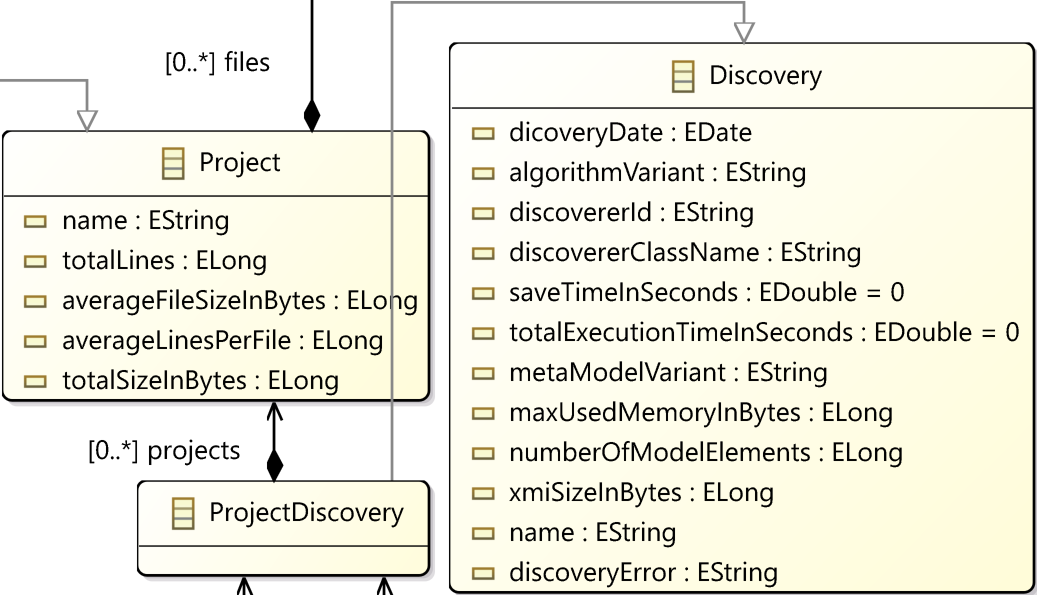
\includegraphics[width=0.48\textwidth]{pics/chapter1pics/example.PNG}
	\caption{Excerpt of Modisco Benchmark metamodel in version 0.9.0.}
	\label{fig: BMM}
	\vspace{-5mm}
\end{figure}

After applying these metamodel changes, naturally, the code of Listing \ref{lis:Modisco_Code_API_V1} is regenerated from the evolved version of the metamodel, which in turn impacts the existing additional code depicted in Listings \ref{lis:Modisco_Code_External_V1}. 
The resulting errors in the original code in version 0.9.0 are underlined in red in Listing \ref{lis:Modisco_Code_External_V1}. 
Listing \ref{lis:Modisco_Code_External_V2} presents the final result of the co-evolution process in version 0.11.0. The co-evolved code is underlined in green. 
For example, in response to the \textit{delete} of the metaclass \texttt{ProjectDiscovery}, its import statement {\small\boxed{Line~1}} in Listing \ref{lis:Modisco_Code_External_V1}, and any usage of it or its methods are impacted. The import statement is completely removed. The same can be applied to the usages of the class and its methods. Alternatively, they could also be replaced by a default value rather than removing the whole instruction. The intention is to maintain the developers' code with minimal removal co-evolution. 

Furthermore, the same changes \textit{rename} and \textit{move} of the property \emph{totalExecutionTimeInSeconds} impact two usages that are co-evolved differently. First, the call of \texttt{setTotalExecutionTimeInSeconds} ({\small\boxed{Line~4}} in Listing~\ref{lis:Modisco_Code_External_V1}) that is co-evolved by renaming it to \texttt{setDiscoveryTimeInSeconds}, then extending the path with \texttt{getIterations()}. The second impact is the use of the generated literal %\texttt{BenchmarkPackage.}\emph{\footnotesize{DISCOVERY\_\_TOTAL\_EXECUTION\_TIME\_IN\_SECONDS}}. It is successively co-evolved by renaming it to \texttt{BenchmarkPackage.}\emph{\footnotesize{DISCOVERY\_\_DISCOVERY\_TIME\_IN\_SECONDS}} before replacing its source class \texttt{DISCOVERY} by \texttt{DISCOVERY\_ITERATION}. 
\texttt{\footnotesize{BenchmarkPackage.DISCOVERY\_\_TOTAL\_EXECUTION\_TIME\_IN\_SECONDS}}. It is successively co-evolved by renaming it to \texttt{\footnotesize{BenchmarkPackage.DISCOVERY\_\_DISCOVERY\_TIME\_IN\_SECONDS}} before replacing its source class \texttt{DISCOVERY} by \texttt{DISCOVERY\_ITERATION}. 
Note that when using the IDE quick fixes to co-evolve these errors, it suggests to create the method \texttt{setTotalExecutionTimeInSeconds} in the class \texttt{Discovery} and the literal \emph{\footnotesize{DISCOVERY\_\_TOTAL\_EXECUTION\_TIME\_IN\_SECONDS}} in the class \texttt{BenchmarkPackage}, which does not meet the required co-evolutions shown in Listing~\ref{lis:Modisco_Code_External_V2}.

The above examples show the importance of correctly matching the different code usages and patterns of the generated code elements with the metamodel evolution changes to co-evolve them with the appropriate resolutions. 

The next section presents our contribution for a fully automatic co-evolution of metamodel and code.  

\begin{lstlisting}[language=Java,breaklines=true,mathescape,literate={\-}{}{0\discretionary{-}{}{}},caption=excertprpt of the generated code in org.eclipse.modisco.infra.discovery.benchmark.\label{lis:Modisco_Code_API_V1}]
	//Discovery Interface
	public interface Discovery extends EObject {
		double getTotalExecutionTimeInSeconds();
		void setTotalExecutionTimeInSeconds(double value);
		...
	}
	//Project Interface
	public interface ProjectDiscovery extends Discovery {...}
	//DiscoveryImpl Class
	public class DiscoveryImpl extends EObjectImpl implements Discovery {
		public double getTotalExecutionTimeInSeconds() {...}
		public void setTotalExecutionTimeInSeconds(double totalExecTime) {...}
		...
	}
\end{lstlisting}
%xleftmargin=0.2cm,xrightmargin=0cm,framexleftmargin=+6pt,frame=single,
\begin{lstlisting}[language=Java,breaklines=true,mathescape,literate={\-}{}{0\discretionary{-}{}{}},caption=Excerpt of the additional code V1.\label{lis:Modisco_Code_External_V1}]
	import (*{\scriptsize org.eclipse.modisco.infra.discovery.benchmark}*).(*\ul{\scriptsize ProjectDiscovery}*);
	public class Report {
		...
		discovery.(*\ul{setTotalExecutionTimeInSeconds}*)(...);
	}
	...
	public class CDOProjectDiscoveryImpl extends AbstractCDODiscoveryImpl implements CDOProjectDiscovery {
		...
		case JavaBenchmarkPackage.
		CDO_PROJECT_DISCOVERY__TOTAL_EXECUTION_TIME_IN_SECONDS: return BenchmarkPackage.
		(*\ul{DISCOVERY\_\_TOTAL\_EXECUTION\_TIME\_IN\_SECONDS}*);
		...
	}
	
	
\end{lstlisting}

\begin{comment}
	public class JavaDiscoveredProjectImpl extends AbstractJavaProjectImpl implements JavaDiscoveredProject {
		
		public int eBaseStructuralFeatureID(int derivedFeatureID, Class<?> baseClass) {
			...
			case JavaBenchmarkPackage.JAVA_DISCOVERED_PROJECT__DISCOVERIES: return BenchmarkPackage.
			(*\ul{DISCOVERED\_PROJECT\_\_DISCOVERIES}*);
			...
		}
		...
	}
\end{comment}
%%%%%%%%%%%%%%%%%%%%%%%%%%%%%%%%%%%%%%%%%%%%%%%%%%%%%%%%%%%
%%                   Now the evolved code                %%
%%%%%%%%%%%%%%%%%%%%%%%%%%%%%%%%%%%%%%%%%%%%%%%%%%%%%%%%%%%
\setulcolor{green} 
\setstcolor{green}
%\setstcolor{green}
%,xleftmargin=0.2cm,,xrightmargin=-0cm,framexleftmargin=+6pt,frame=single
\begin{lstlisting}[language=Java,breaklines=true,mathescape,literate={\-}{}{0\discretionary{-}{}{}},caption=Excerpt of the additional code V2.\label{lis:Modisco_Code_External_V2}]
	(*{\st{import }}*)(*{\scriptsize \st{ org.eclipse.modisco.infra.discovery.benchmark. ProjectDiscovery}}*);
	public class Report {
		...
		discovery.(*\ul{getIterations().}*) 
		(*\ul{setDiscoveryTimeInSeconds}*)(...);
		...
	}
	public class CDOProjectDiscoveryImpl extends AbstractCDODiscoveryImpl implements CDOProjectDiscovery {
		...
		case JavaBenchmarkPackage.
		CDO_PROJECT_DISCOVERY__TOTAL_EXECUTION_TIME_IN_SECONDS: return BenchmarkPackage.
		(*\ul{DISCOVERY\_ITERATION\_\_DISCOVERY\_TIME\_IN\_SECONDS}*);
		...
	}
	...
}
\end{lstlisting}
%\begin{lstlisting}[language=Java,breaklines=true,mathescape,literate={\-}{}{0\discretionary{-}{}{}},xleftmargin=0.2cm,xrightmargin=-0.4cm,framexleftmargin=+6pt,frame=single,caption=Excerpt of the additional external code in the SL org.eclipse.modisco.infra.discovery.benchmark.\label{lis:Modisco_Code_External_V1}]

\begin{comment}
....
public class JavaDiscoveredProjectImpl extends AbstractJavaProjectImpl implements JavaDiscoveredProject {
	public int eBaseStructuralFeatureID(int derivedFeatureID, Class<?> baseClass) {
		...
		case JavaBenchmarkPackage.JAVA_DISCOVERED_PROJECT__DISCOVERIES: return BenchmarkPackage.(*\ul{BENCHMARK\_\_DISCOVERIES}*);
		...
	}
	...
}
\end{comment}



\section{Approach}\label{approach}

This section presents the overall approach of our automated co-evolution of code with evolving metamodels,  instantiating on the Ecore technological space. First, we give an overview of the approach and specify the metamodel evolution changes we consider. 
%
Then, we present how we retrieve the resulting errors due to metamodel evolution, followed by the regeneration of the code API. 
After that, we present the pattern matching process, which is an important part of our fully automatic co-evolution approach, before discussing the resolutions of the code errors. 

\subsection{Overview}
\label{Overview}
Figure~\ref{fig:overallapproach} depicts the overall steps for the automatic co-evolution of the metamodel and code, with horizontally separated parts defining chronological order from the top to the bottom.
%\\
After the generation step (the upper part of Figure~\ref{fig:overallapproach}), the evolution of the Ecore metamodel will cause errors in the additional Java code that depends on the API of the newly generated code (the middle part of Figure~\ref{fig:overallapproach}). We take as input the evolution changes of the metamodel between the two versions of this metamodel {\small\boxed{1}}. Then, we parse the additional code  {\small\boxed{2}} to retrieve the list of errors. 
After that, we get to the bottom part of Figure~\ref{fig:overallapproach}, both the list of metamodel changes and the list of errors are used as inputs for the \red{pattern matching step {\small\boxed{3}}. It analyzes the structure of the error to match it with its impacting metamodel change and decides which resolution  {\small\boxed{4}} to apply for the error co-evolution {\small\boxed{5}}. The metamodel changes provide the ingredients and necessary information that are used for the co-evolution.  
	At the end of the automatic co-evolution, we obtain a new co-evolved additional code {\small\boxed{6}} along a generated report on the applied resolutions.} 
In addition to the automatic co-evolution, we generate test cases before and after co-evolution to highlight its possible effect. In fact, many research papers rely on the use of tests to check the behavior of the code during its evolution. For example, Godefroid et al.~\cite{10.1145/3395363.3397374} uses tests to find regressions in different versions of REST APIs. In particular, Lamothe et al.~\cite{9079197},~\cite{10.1145/3387905.3388608} use tests to validate the evolution of the client code after Android API migration. We apply a similar method to check the effect of the co-evolution. 
Finally, during the co-evolution process, we generate a report linking the applied resolutions for each code error with its impacting metamodel change. If needed, this can help developers in understanding the performed co-evolution, since we fully automate it.
%\todo{refs behavioral check et papier android : to check}
%\DK{we see later if we add the story of generated tests after co-evolution}

\subsection{Metamodel Evolution Changes}
\label{mmchanges}

One of the intrinsic properties of software artifacts is its continuous evolution~\cite{mens2008introduction}. Metamodels are no different and are meant to evolve. 
Two types of evolution changes are considered when evolving a metamodel: \emph{atomic} and \emph{complex} changes~\cite{Herrmannsdoerfer2011}. 
Atomic changes are additions, removals, and updates of a metamodel element. Complex changes consist of a sequence of atomic changes combined together~\cite{vermolen_reconstructing_2012},~\cite{khelladi2015detecting}. For example, move property is a complex change where a property is moved from a source class to a target class. This is composed of two atomic changes: delete property and add property~\cite{Herrmannsdoerfer2011}. 
Many approaches in the literature~\cite{Alter2015, williams2012searching,cicchetti_managing_2009,langer_posteriori_2013,vermolen_reconstructing_2012,Khelladi2016,bettini2022executable} exist to detect metamodel changes between two versions. Note that the detected list of complex changes does not include the list of the detected atomic changes, i.e., no overlap in between. 
\red{Moreover, the detection approaches must order the changes in a consistent way. This is fundamentally a problem that change detection approaches must deal with, and hence, is out of scope for our problem of code co-evolution. Nonetheless, it is important and expect a consistent order of changes to not hinder the quality of the co-evolution.}

For the purpose of modularity and extensibility, we use a specification layer for the changes~{\small\boxed{1}} that is simply a connection layer to our co-evolution approach with existing change detection approaches. This connection layer specifies our own representation of a metamodel change that can be mapped later with any change representation. \red{It simply specifies the needed information for each change in the form of its attributes. In the left column of Table \ref{table:ResolutionsCatalog}, we precise the impacting changes that we consider in our work. For each change, we precise in the second column the attributes that represent and compose each change. When using a state-of-the Art detection approach, we analyze in white box the detected changes to extract their attributes and map them to our internal change layer.
	%the attributes of each change are mapped with the corresponding detected change. In order to map the output changes of the used detection approach, we analyze in white box their results to retrieve their different attributes and map them with our change layer.
} 
For example, a rename property change includes information regarding its old name, new name, and its class container. Therefore, in practice, any detection approach~\cite{Alter2015, williams2012searching,cicchetti_managing_2009,langer_posteriori_2013,vermolen_reconstructing_2012,Khelladi2016,bettini2022executable} can be integrated by bridging its changes' representation to our change layer and the rest of co-evolution can be performed independently.
In this approach, we chose to reuse our previous work \cite{Khelladi2016}, a heuristic-based approach to actually detect atomic and complex changes between two versions of a metamodel.
In the rest of the chapter, we focus on the code co-evolution since it is our main contribution. 

\subsection{Error Retrieval}
\label{errorretrieving}

After the metamodel is evolved and the code API is re-generated, errors will appear in the additional code that must be co-evolved. Unlike code migration context~\cite{9079197},~\cite{henkel2005catchup}, these errors represent the delimited impact of the metamodel evolution. Thus, rather than an impact analysis on the original version to trace the impact of a metamodel change in the code, our approach relies on the compilation result of the code to retrieve its errors. 
This is necessary and useful in our approach, as we will need to keep updating the list of code errors after co-evolving each given error, hence, iteratively co-evolving the code. We detail this process in the following subsections.

To retrieve those errors, we start by parsing the code of each Java class, called a \emph{compilation unit}, to access the Abstract Syntax Trees (ASTs). An error in a Java code is called a \emph{Marker} that contains the information regarding the detected error. It contains the necessary information to locate the exact impacted AST node in the parsed global AST (\ie char start and end) and  to process it (\ie message).
In the remaining part of the chapter, instead of Markers, compilation units, and additional code, we respectively refer only to errors, Java classes, and code for the sake of simplicity.  

\subsection{Resolution Catalog}

Now that we have a list of code errors, we need a set of resolutions to co-evolve them.
\blue{Our co-evolution approach relies on the resolutions shown in Table \ref{table:ResolutionsCatalog}. 
	%
	%Table \ref{table:ResolutionsCatalog} 
	It depicts the resolutions associated with metamodel changes that are known to have an impact on code \cite{iovino2012impact}.
	The resolutions are taken from existing co-evolution approaches of various MDE artifacts \cite{kessentini2018integrating,kessentini2019automated,cicchetti2008automating,herrmannsdoerfer2009cope,garces2009managing,wachsmuth2007metamodel,batot2017heuristic,khelladi2017semi,correa2007refactoring,kessentini2018automated,khelladi2018change,garces2014adapting,garcia2013model,kusel2015consistent,kusel2015systematic,hebig2015surveying}, % or constraints \cite{khelladi2017semi}
	where they showed to be efficient and useful in co-evolving code \cite{Khelladi2020}.
	
	For example, resolutions $[CR8,CR9, CR10, CR11]$   aim to co-evolve the different code errors of a move property in the metamodel. %We notice that a metamodel change can be treated by more than one resolution, so how do we select one resolution per change? [or the following paragraph presents our solution to select one resolution per change.]
}


\begin{sidewaystable}


	%\setlength\extrarowheight{1pt}
%\begin{table*}[t]
	%\vspace{-1.5em}
	\centering

	\caption{Catalog of resolutions used for the code co-evolution of direct errors due to the metamodel changes.}
	\label{table:ResolutionsCatalog}
	\resizebox{22.5cm}{!} {
	%	\vspace{-4cm}
			\hspace{-1cm}

		\begin{tabular}{lll}
			\toprule
			\begin{tabular}[c]{@{}l@{}}Impacting Metamodel Changes\end{tabular} 
			&  \begin{tabular}[c]{@{}l@{}}Changes' attributes\end{tabular} 
			& \begin{tabular}[c]{@{}c@{}}Proposed Code Resolutions\end{tabular}   
			
			\\ \midrule
			
			
			
			%			* 0 to delete the instruction where the deleted method is used, 
			%			* 1 delete the direct element only 
			%			* 2 delete the direct expression (all call path) using this deleted property 
			%			* 3 replace the direct expression (all call path) with a default value
			%			* 4 replace it with another element (like rename)
			
			\begin{tabular}[c]{@{}l@{}}	$\diamond$ Delete property \emph{p} \\from class \emph{C}\end{tabular} 
			&  \begin{tabular}[c]{@{}l@{}}	$\circ$ Property \emph{p} name \\ $\circ$ Container class \emph{C} name\end{tabular} &  
			\begin{tabular}[c]{@{}l@{}}$\rhd [CR1]$ Remove the direct use of \emph{p} \red{}(e.g., label = s.name + s.m1().p.m2() $\rightarrow$ label = s.name + ( (Type\_Of\_P) s.m1() ).m2())\\
				$\rhd [CR2]$ Remove the statement using \emph{p} (i.e., if, loop, assignment, etc.) \\
				$\rhd [CR3]$ Remove the whole call path of \emph{p} (e.g., label = s.name + s.m1().m2().p $\rightarrow$ label = s.name) \\
				$\rhd [CR4]$ Replace the whole call path of \emph{p} with a default value (e.g., id = s.id + s.m1().m2().p $\rightarrow$ id = s.id + 0) 
				
			\end{tabular}    \\ \midrule
			
			$\diamond$ Delete class \texttt{C} 
			& \begin{tabular}[c]{@{}l@{}}$\circ$ Class \emph{C} name \\ $\circ$ Container package \emph{Q} name\end{tabular} 
			& \begin{tabular}[c]{@{}l@{}}$\rhd [CR1]$ Remove the direct use of the type \texttt{c} (e.g., extending/implementing \texttt{c}, in method argument/returned \\ type and not the whole method declaration. Calls to the updated methods are subsequently updated) \\%\textcolor{white}{-----------}
				$\rhd [CR2]$ Remove the statements using the type \texttt{C} (e.g., import, variable declaration, method argument/returned type, \\ method declaration,  type instantiation, etc. Calls to the deleted variables and methods are subsequently removed)\\%\textcolor{white}{-----------}
				
			\end{tabular} 	  \\ \midrule
			
			$\diamond$ Rename element \emph{e} to \emph{e'}
			& \begin{tabular}[c]{@{}l@{}}	$\circ$ Element \emph{e} old name \\$\circ$ Element \emph{e'} new name \\$\circ$ Container package \emph{Q} or class \emph{C} name\end{tabular}
			& \begin{tabular}[c]{@{}l@{}} $\rhd [CR5]$ Rename \emph{e} in the code	
			\end{tabular}
			\\
			\midrule
			
			\begin{tabular}[c]{@{}l@{}}$\diamond$ Generalize multiplicity of \\ property \emph{p} of the class \emph{C} from \\ a single to multiple values\end{tabular} 
			& \begin{tabular}[c]{@{}l@{}}	$\circ$ Property \emph{p} name \\ $\circ$ Container Class  \emph{C} \\ $\circ$ Old multiplicity
				\\ $\circ$ New multiplicity\end{tabular} 
			& 
			\begin{tabular}[c]{@{}l@{}}
				$\rhd [CR6]$ Retrieve the first value of a collection (e.g., value = \emph{lng.p}  $\rightarrow$ value = \emph{lng.p.toArray()[0]} or \emph{lng.p.get(0)} )\\
				
			\end{tabular}   \\ \midrule
			
			%			* 0 extend navigation path
			%			* 1 reduce navigation path
			%			* 2 extend a navigation path and add a loop
			%			* 3 extend a navigation path and get the first/last/i^th element
			%			* 4 replace reference in path call x.y.z.prop to x.y.w.prop
			
			\begin{tabular}[c]{@{}l@{}}$\diamond$ Move property $p_{i}$ from \\ class \texttt{S} to \texttt{T} through \emph{ref}\\
				%$\diamond$ Extract class \texttt{S} to \texttt{T} \\with properties $p_{1},...,p_{n}$ \\ \red{through \emph{ref}}\\
				$\diamond$ Extract class of properties $p_{1},$\\$...,p_{n}$ from \texttt{S} to \texttt{T} through \emph{ref}\end{tabular}
			& \begin{tabular}[c]{@{}l@{}} $\circ$ Property \emph{p} name \\ $\circ$ Source container class \emph{S} name \\$\circ$  Target container class \emph{T} name \\$\circ$ Reference \emph{ref} name \end{tabular} 
			& 
			\begin{tabular}[c]{@{}l@{}}$\rhd [CR7]$ Extend navigation path of $p_{i}$ (e.g., \emph{lng.$p_{i}$}  $\rightarrow$ \emph{lng.ref.$p_{i}$})\\
				
				$\rhd [CR8]$ Extend navigation path of $p_{i}$ and add a for loop (e.g., \emph{lng.$p_{i}$}  $\rightarrow$ \emph{for(v in lng.ref) \{v.$p_{i}$\}})\\
				$\rhd [CR9]$ Reduce navigation path of $p_{i}$ (e.g., \emph{lng.ref.$p_{i}$}  $\rightarrow$ \emph{lng.$p_{i}$})\\
				$\rhd [CR10]$ Replace S by T\_REF  in Literal values (e.g., \emph{MetamodelPackage.S\_\_$p_{i}$}  $\rightarrow$ \emph{MetamodelPackage.T\_\_$p_{i}$})
			\end{tabular}   \\ \midrule
			
			\begin{tabular}[c]{@{}l@{}}$\diamond$ Push property \emph{p} from \\class \texttt{Sup} to \texttt{Sub$_{1}$},...,\texttt{Sub$_{n}$}\end{tabular} 
			& \begin{tabular}[c]{@{}l@{}}	$\circ$ Property \emph{p} name \\ $\circ$ Container class \emph{Sup} name \\ $\circ$ List of container classes \emph{Sub$_{i}$} names
			\end{tabular} 
			& 
			\begin{tabular}[c]{@{}l@{}}$\rhd [CR11]$ Introduce a type test with an If statement (e.g., \emph{t.name = s.p.name} $\rightarrow$ \\$if(s.p.istypeof(Sub_{1})$) \{t.name = (Sub$_{1}$ s).p.name\} $...$ $else$ $if(s.p.istypeof(Sub_{n})$ \{t.name = (Sub$_{n}$ s).p.name\})\\
				$\rhd [CR12]$ Cast \emph{p} to one specific sub class $Sub_{i}$ (e.g., \emph{t.name = s.p.name} $\rightarrow$ \emph{t.name = (($Sub_{i}$)s).p.name})\\
				$\rhd [CR13]$ Duplicate the statement using the literal for each subclass and replace Sup by $Sub_{i}$ (e.g., \emph{add(Package.Sup\_\_P)} \\ $\rightarrow$ \emph{ add(Package.$Sub_{0}$\_\_P)}, ... , \emph{add(Package.$Sub_{n}$\_\_P)})
				%Create much Literals as subclasses and replace Sup by $Sub_{i}$ in each one(e.g., \emph{MetamodelPackage.Sup\_\_P}  $\rightarrow$ \emph{lng.$Sub_{0}$\_\_P} ,...,\emph{lng.$Sub_{n}$\_\_P})
			\end{tabular}   \\ \midrule
			\begin{tabular}[c]{@{}l@{}}$\diamond$ Pull property \emph{p} from \\classes \texttt{Sub$_{1}$},...,\texttt{Sub$_{n}$}
				to \texttt{Sup}  \end{tabular} 
			& \begin{tabular}[c]{@{}l@{}}		$\circ$ Property \emph{p} name \\ $\circ$ List of container classes \emph{Sub$_{i}$}  \\ $\circ$ Container class \emph{Sup} name\end{tabular} 
			& 
			\begin{tabular}[c]{@{}l@{}}
				%$\rhd [CR12]$ Cast \emph{p} to sup  (e.g., \emph{t.name = s.p.name} $\rightarrow$ \emph{t.name = ((Sup)s).p.name})\\
				$\rhd [CR14]$ Replace $Sub_{i}$  by Sup in Literal values (e.g., \emph{MetamodelPackage.$Sub_{i}$\_\_P}  $\rightarrow$ \emph{MetamodelPackage.Sup\_\_P})
				
			\end{tabular}   \\ \midrule
			
			%			\begin{tabular}[c]{@{}l@{}}$\diamond$ Extract class \texttt{S} to \texttt{T} \\with properties $p_{1},...,p_{n}$\end{tabular} & 
			%			\begin{tabular}[c]{@{}l@{}}$\rhd [CR10]$ Extend navigation path of $p_{i}$ (e.g., \emph{lng.$p_{i}$}  $\rightarrow$ \emph{lng.path.$p_{i}$})\\
				%				$\rhd [CR11]$ Reduce navigation path of $p_{i}$ (e.g., \emph{lng.path.$p_{i}$}  $\rightarrow$ \emph{lng.$p_{i}$}) \end{tabular}   \\ \midrule
			
			%			
			
			
			\begin{tabular}[c]{@{}l@{}}$\diamond$ Inline class \texttt{S} to \texttt{T} \\with properties $p_{1},...,p_{n}$\end{tabular} 
			& \begin{tabular}[c]{@{}l@{}}   $\circ$ List of properties \emph{p$_{i}$}  \\$\circ$ Container Source class \emph{S} name \\ $\circ$ Container Target class \emph{T} name\end{tabular} 
			& 
			%delete rule or change its source/target type from B to A
			\begin{tabular}[c]{@{}l@{}}
				$\rhd [CR9]$ Reduce navigation path of $p_{i}$ (e.g., \emph{lng.ref.$p_{i}$}  $\rightarrow$ \emph{lng.$p_{i}$})\\
				$\rhd [CR15]$ Change the class type from \texttt{S} to \texttt{T} \red{}(e.g., List$<$S$>$ l = ...; $\rightarrow$ List$<$T$>$ l = ...; ) \\
			\end{tabular} \\ \midrule
			
			%			\begin{tabular}[c]{@{}l@{}}$\diamond$ Flatten hierarchy from \\class \texttt{Sup} to \texttt{Sub$_{1}$},...,\texttt{Sub$_{n}$}\\with properties $p_{1},...,p_{n}$\end{tabular} & 
			%			%delete rule of change its source/target type from A to B1 ... Bn
			%			\begin{tabular}[c]{@{}l@{}}$\rhd [R15]$ Duplicate the transformation rule while changing the source or target class type from \texttt{Sup} to \texttt{Sub$_{i}$} ($i \in [1...n] $)  \\
				%				$\rhd [CR3]$ Remove the whole transformation rule \\ \end{tabular}  \\ 
			\begin{tabular}[c]{@{}l@{}}$\diamond$ Change property \emph{p} type \\ of the class \emph{C} from \texttt{S} to \texttt{T}\end{tabular}
			& \begin{tabular}[c]{@{}l@{}}	$\circ$ Property \emph{p} name \\ $\circ$ Container class \emph{C} name \\ $\circ$ Old type \emph{S}\\ $\circ$ New type \emph{T} \end{tabular} 
			& 
			\begin{tabular}[c]{@{}l@{}}$\rhd [CR16]$ Change variable declaration type initialized with \emph{p} from \texttt{S} to \texttt{T} (e.g., S var = s.p; $\rightarrow$ T var = s.p;) \\ $\rhd [CR17]$ Add a cast of \emph{p} 
			\end{tabular}   \\ %\midrule
			\bottomrule  
			
			                
		\end{tabular}
				
}
%\end{adjustbox}	
\end{sidewaystable}	
%\end{table*}


\subsection{Pattern Matching for Resolution Selection}
\label{pattern_matching}



\begin{table*}[t]
	
	\caption{Classification of the different patterns of the generated code element from the metamodel elements.} 
	\label{table:locationofMMelemen_ch1}
	\hspace{-1cm}
	\resizebox{19cm}{!} {
		{\small
			\begin{tabular}{llll}
				\toprule
				
				\begin{tabular}[c]{@{}l@{}} \textbf{Metamodel}\\ \textbf{element type} 
				\end{tabular} & \textbf{Generated code elements}& \textbf{Pattern of the generated code elements}& \textbf{Illustrative examples}\\ \midrule
				
				
				\multirow{6}{*}{Metaclass} & Interface & "MetaClassName" & \textit{Constraint} \\ \cline{2-4} 
				& \begin{tabular}[c]{@{}l@{}}createClass() \\ (in metamodelFactory class)\end{tabular} & "create"+"MetaClassName"() &\textit{createConstraint()} \\ \cmidrule{2-4} 
				& \begin{tabular}[c]{@{}l@{}}Literals of the class \end{tabular} &
				\begin{tabular}[c]{@{}l@{}}
					"META\_CLASS\_NAME"\\
					"META\_CLASS\_NAME"+"\_"+ "FEATURE\_COUNT"\\
					"META\_CLASS\_NAME"+ "\_"+"OPERATION\_COUNT"
				\end{tabular} 
				& \begin{tabular}[c]{@{}l@{}}\textit{CONSTRAINT}, \\ \textit{CONSTRAINT\_FEATURE\_COUNT}, \\  \textit{CONSTRAINT\_OPERATION\_COUNT}\end{tabular} \\ \cmidrule{2-4} 
				& \begin{tabular}[c]{@{}l@{}}Accessor of Meta objects \\ (in metamodelPackage class)\end{tabular} & "get"+"MetaClassName"()& \textit{getConstraint() }\\ \cmidrule{2-4} 
				& Class implementation & "MetaClassNameImpl" &\textit{ConstraintImpl }\\ \cmidrule{2-4} 
				& Adapter & "create"+"MetaClassName"+"Adapter" & \textit{createConstraintAdapter()} \\ \midrule
				
				
				\multirow{1}{*}{Attribute} & Signature of getters and setters & "get"+"AttributeName"(), "set"+"AttributeName"()& \textit{getStereotype()}, \textit{setStereotype() }\\ \cmidrule{2-4} 
				\multirow{3}{*}{(same for a reference)} & Accessor of Meta objects &"get"+"MetaClassName"+"\_"+"AttributeName"() &\textit{ getConstraint\_Stereotype()} \\ \cmidrule{2-4} 
				& Literal & "META\_CLASS\_NAME"+"\_\_"+"ATTRIBUTE\_NAME"& \textit{CONSTRAINT\_\_STEREOTYPE} \\ \cmidrule{2-4} 
				& \begin{tabular}[c]{@{}l@{}}Implementation \\ of getters and setters\end{tabular} &"get"+"AttributeName"(), "set"+"AttributeName"()& getStereotype(), setStereotype() \\ \midrule
				
				
				\multirow{4}{*}{Method} & Declaration of the method& "methodName"()& \textit{UniqueName() }\\ \cmidrule{2-4} 
				& Accessor of meta objects &"get"+"MetaClass"+"\_\_"+"MethodName"()& \textit{getCONSTRAINT\_\_UniqueName() }\\ \cmidrule{2-4} 
				& Literal &"META\_CLASS\_NAME"+"\_\_"+"METHOD\_NAME"& \textit{CONSTRAINT\_\_\_UNIQUE\_NAME }\\ \cmidrule{2-4} 
				& Implementation of the method &"methodName"()& \textit{UniqueName()} \\ %\midrule
				
				
				%\multirow{4}{*}{Reference} & Accessor of meta objects &"get"+"MetaClassName"+"\_"+"ReferenceName"()& \textit{getConstraint\_ConstraintElement()} \\ \cmidrule{2-4} 
				% & Signature of getters and setter & "get"+"ReferenceName"(),"set"+"ReferenceName"()&\textit{ getConstraintElement()}, \textit{setConstraintElement() }\\ \cmidrule{2-4} 
				% & Literal &"META\_CLASS\_NAME"+"\_\_"+"REFERENCE\_NAME"& \textit{CONSTRAINT\_\_CONSTRAINT\_ELEMENT} \\ \cmidrule{2-4} 
				% & \begin{tabular}[c]{@{}l@{}}Implementation of \\ getters and setters\end{tabular} &"get"+"ReferenceName"(), "set"+"RegerenceName"()& \textit{getConstraintElement()}, \textit{setConstrainElement() }\\ 
				\bottomrule
				
				%cline hline replaced with cmidrule and midrule
				
			\end{tabular}
		}
	}
\end{table*}

As shown in Table \ref{table:ResolutionsCatalog}, alternative resolutions exist per metamodel change. Since we aim to fully automate the co-evolution, we need a mechanism to analyze the code error, the code usage, and its impacting metamodel change to decide which resolution to apply. 
This section presents the pattern matching process between metamodel changes and code usages for the retrieved code errors to automatically select resolutions for their co-evolution.

Each Metamodel Element $ME$ has corresponding Generated Code Elements \{$GCE_0$, $GCE_1$, ..., $GCE_n$\} in the code API. 
$GCE_i$ have \textbf{usages} in the \textbf{additional code} as illustrated in Figure~\ref{fig:patternconcept}.
Thus, evolving a $ME$ will regenerate \{$GCE_0$, $GCE_1$, ..., $GCE_n$\} which will impact their \textbf{usages}. 
%
Table~\ref{table:locationofMMelemen} classifies the different patterns of the generated code elements $GCE_i$ for each metamodel element $ME$ type, and provides illustrative examples. It shows that various patterns of code elements are generated for each metamodel element type. % and with different patterns. 
%mapping between the different metamodel elements and their corresponding generated code elements with illustrative examples. 
For example, let us consider the case of a metaclass. EMF generates a corresponding interface and a class implementation, a \emph{createClass()} method in the factory class, three literals (\ie constants) for the class and an accessor method in the package class, and a corresponding create adapter method. For the attribute case, EMF generates the signature and implementation of a getter and a setter, an accessor method in the package class, and a literal. 

This classification is essential to match the different code errors with their corresponding \textbf{pattern} of the $GCE_i$ in Table~\ref{table:locationofMMelemen}. 
%
Moreover, each generated code element $GCE_i$ can be used in different \textbf{configurations} in the code that must also be considered in the pattern matching process. For example, using a $GCE_i$ as a parameter in a method declaration and in a method invocation, or to initialize a variable declaration, or in an expression call in a statement, etc., are considered as different configurations and can influence which resolution to apply as well. With these ingredients, we can match a resolution for each error. 
%\red{For example, from the attribute \emph{totalExecutionTimeInSeconds} in the class \texttt{Discovery} in Figure \ref{fig:overallapproach}, a setter method (i.e., pattern) is generated in Listing \ref{lis:Modisco_Code_API_V1} (line~12) and has a usage in the code of Listing \ref{lis:Modisco_Code_External_V1} (line 4) in a call expression statement (i.e., configuration). 
	%Thus, to be able to select the appropriate resolution for the code co-evolution, we must match the pattern of the $GCE_i$ and its configuration usage in the code error with the impacting metamodel change.} 

\red{
	%To sum up, an error is finally an impacted usage of a $GCE_i$.
	%\textbf{A pattern} is a (data) structure that associates an error, in the additional code, to its causing change and the configuration of its corresponding $GCE_i$ usage, so that it facilitates the selection of a resolution for this error.
	%The information about the causing change is not sufficient because, as shown in Table \ref{table:ResolutionsCatalog}, a change can be associated to more than one resolution, we need more information to better select only one resolution automatically. After analyzing different types of changes and resulting errors, we found that the configuration of the usage of a $GCE_i$ allows us to pre-select the appropriate resolution. The resolution in our approach is a resolution that favors minimum deletion, and minimum side effect errors.
	
	%Let us take an example of push property change. It has three possible resolutions: CR11, CR12 and CR13. Assuming that we have an error for which we aim to find a resolution. Our pattern matching process starts by parsing the error to link it with the causing change. The next step is to define the corresponding type of GCE usage. If it is a literal, the detected pattern is " pushProperty_Literal" implying that the selected resolution will be CR13. For any other usage type, the detected pattern is "pushProperty_notLiteral", the selected resolution in this case is CR11 because it will cover all the possible subclasses.
	%Let us take the example of \texttt{"Change property type from S to T"} (last change type in Table \ref{table:ResolutionsCatalog}). It has two possible resolutions, CR16 and CR17. Assuming that we have a code error that must be co-evolved. Our pattern matching process first identifies the pattern of the corresponding $GCE_i$ from Table~\ref{table:locationofMMelemen} (line 6), then the configuration of the $GCE_i$ usage (Lines 7-13). 
	%starts by parsing the error to find the pattern of the corresponding $GCE_i$, which will help to find the causing change. The next step is to define the configuration of the $GCE_i$ which means the type of the $GCE_i$ usage. 
	%If it is a variable declaration (line 8), the resolution $CR16$ is returned. If any other configuration is detected, the pattern matching process returns $CR17$ as an appropriate resolution. 
	
	
}
\begin{figure}[t]\centering%
	%\hspace*{-1cm}
	%\centering
	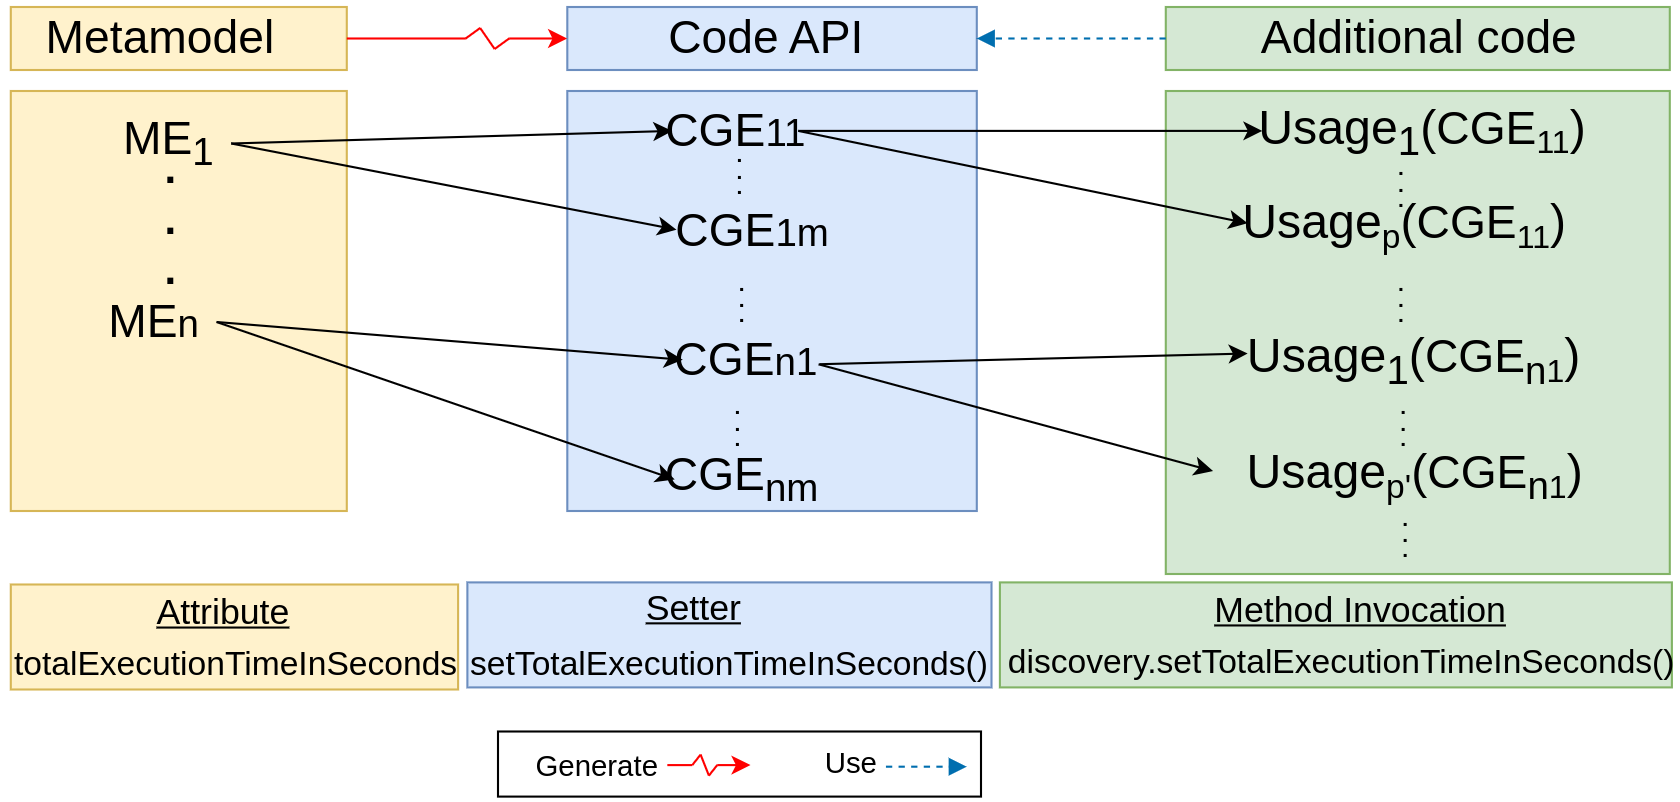
\includegraphics[width=0.5\textwidth]{pics/chapter1pics/patternusages.png}
	\caption{Schema for mapping between the metamodel and code.}
	\label{fig:patternconcept}
	\vspace{-1em}
	
\end{figure}

Algorithm \ref{algo :ErrorPatternalgo} summarizes the pattern matching process. 
Given a Java class, an error, and a list of metamodel changes, Algorithm~\ref{algo :ErrorPatternalgo} first retrieves the error AST node~{\small\boxed{line~2}}. After that, it identifies the configuration of the $GCE$ usages~{\small\boxed{Line~3}}. Then, for each metamodel change type ~{\small\boxed{lines~6,17,22,31}}, it identifies the pattern of the corresponding $GCE$ presented in Table~\ref{table:locationofMMelemen}~{\small\boxed{line~7,18,23,32}}. %the different cases of usages in the additional code~{\small\boxed{Lines~3, 2}}, \eg \emph{SimpleName}, \emph{QualifiedName}, \emph{SingleVariable}, \emph{MethodDeclaration}, etc, which are AST node types depending on its level and its position in the AST of the Java class. 
%Then, it matches it with the metamodel change causing its error~{\small\boxed{Lines ~5, 15, 18}}. This process is applied for the rest of the metamodel changes. 
%When the algorithm finds the causing change, it starts to find the 
Depending on the detected configuration, the appropriate pre-selected resolution is added to the output set~{\small\boxed{Line~10,13,19,26,35}}.
Finally, the selected resolutions set is returned for further processing in the automatic co-evolution~{\small\boxed{Line~41}}. 
Let us take the example of \texttt{"Change property type from S to T"} (last change type in Table \ref{table:ResolutionsCatalog}). It has two possible resolutions, CR16 and CR17. Assuming that we have a code error that must be co-evolved. Our pattern matching process first identifies the pattern of the corresponding $GCE_i$ from Table~\ref{table:locationofMMelemen} (Line 7), then the configuration of the $GCE_i$ usage (Lines 8). 
Algorithm \ref{algo :ErrorPatternalgo} starts by parsing the error to find the pattern of the corresponding $GCE_i$, which will help to find the causing change. The next step is to define the configuration of the $GCE_i$ which means the type of the $GCE_i$ usage. 
If it is a variable declaration (line 9), the resolution $CR16$ is returned. If any other configuration is detected, the pattern matching process returns $CR17$ as an appropriate resolution.

Note that an error can be matched with more than one resolution because a metamodel element $ME$ can be impacted by more than one change, in other terms interdependent changes. 
For example, \red{Algorithm~\ref{algo :ErrorPatternalgo} allows matching the error in~{\small\boxed{Line 17}} (rename property) and ~{\small\boxed{Line 31}} (move property) with two metamodel changes of the property \emph{totalExecutionTimeInSeconds} in Listing~\ref{lis:Modisco_Code_External_V1}.} The generated literal, which is our generated code element $GCE_i$, is used here in the configuration of a literal static field access 
\emph{\footnotesize{BenchmarkPackage.DISCOVERY\_\_TOTAL\_EXECUTION\_TIME\_IN\_SECONDS}}. The returned resolutions are $CR5$ and $CR10$~{\small\boxed{Line 19,35}}, \red{to be executed in the order of detection of their causing metamodel changes.}%\red{Empirically, we observe only the case of interdependency between a rename and move/pull/push changes.}

%Note that several patterns can be matched for a given error caused by multiple changes.
%For example, in Listing~\ref{lis:Modisco_Code_External_V1}, Algorithm~\ref{algo :ErrorPatternalgo} allows to match the error in~{\small\boxed{line 6}} with two patterns caused by the two metamodel changes rename and move of the property \emph{totalExecutionTimeInSeconds}. The generated literal, which is our generated code element $GCE_i$, used here in a static field access, 
%\emph{\footnotesize{BenchmarkPackage.DISCOVERY\_\_TOTAL\_EXECUTION\_TIME\_IN\_SECONDS}}. The matched patterns are \texttt{RenameProperty\_Literal} and \texttt{MoveProperty\_Literal}. %\texttt{RenameProperty\_ SimpleName\_Literal} and \texttt{MoveProperty\_SimpleName\_Literal}. 
%In total, we define 33 patterns that we match with the code usages and metamodel changes. We attach their list as a supplementary material\footnote{\url{https://figshare.com/s/8986914e924300be77da}}.
%Due to lack of space we attach their list as a supplementary material.



A similar mechanism is implemented for the rest of metamodel changes to select a resolution based on the pattern of $GCE_i$ and the configuration of its usage. % ~{\small\boxed{Lines 40-42}}.
For the sake of readability, Algorithm \ref{algo :ErrorPatternalgo} does not show all possible combinations of $metamodel$ $changes \times patterns \times configurations$, but few examples to illustrate its essence. \red{We nonetheless give an extended version in the appendix}

%
Finally, in our implementation, for the case of a "Delete Class" and "Delete Property", we favor the least deletion when possible. In particular, depending on the configuration usage, we select the resolution that deletes the least possible among $CR1$, $CR2$, $CR3$, $CR4$. For example, for an error in a parameter of a method call, we select the resolution $CR4$ rather than $CR1$ or $CR2$. 
In Listing \ref{lis:Modisco_Code_External_V1}, Algorithm \ref{algo :ErrorPatternalgo} matches the error in the import declaration (\textbf{Configuration}), with the deletion of the metaclass \textit{ProjectDiscovery} (\textbf{pattern}), which allows to select the resolution $CR2$.

%However, this is an implementaion strategy and could  

%For example, in Listing \ref{lis:Modisco_Code_External_V1}, the marker in {\small\boxed{line 6}}  \ie
%\texttt{BenchmarkPackage.} \emph{DISCOVERY\_\_TOTAL\_EXECUTION\_TIME\_IN\_SECONDS}  which is a static field access presents an erroneous usage of the $GCE_i$  Literal of an attribute caused by the metamodel change rename the property \emph{totalExecutionTimeInSeconds} to \emph{discoveryTimeInSeconds}. Algorithm \ref{algo :ErrorPatternalgo} allows to match it  with the pattern RenameProperty\_SimpleName\_Literal.


\definecolor{circlegreen}{HTML}{7ed321}



\begin{algorithm2e}[t]
	% \algsetup{linenosize=\tiny}
	\small
	
	\SetAlgoLined
	\KwData{javaClass, error, changesList}
	
	resolution\_s $\leftarrow \phi$ 
	
	%\While{(!usage.hasPatterns())}
	%{
		errorNode $\leftarrow$ findErrorAstNode(javaClass, error)
		
		configuration $\leftarrow$ getConfiguration(javaClass,errornode)
		
		%change $\leftarrow$ changesList.next()
		
		\For {(change  $\in$ changesList)}
		{
			\Switch{change}{
				\Case{ChangePropertyType}{
					\uIf{(match(patternGCE,change)}
					{
						
						\Switch{configuration}{
							
							\Case{VariableDeclaration}{
								
								resolution\_s.add("CR16")
							}
							
							\Other{
								
								resolution\_s.add("CR17")
							}
							
							
							
						}
					}
					
					
				}
				
				\Case{RenameProperty}{
					\uIf{(match(patternGCE,change)}
					{
						%configuration $\leftarrow$ getConfiguration(javaClass,errornode)
						
						resolution\_s.add("CR5")
						
					}
					
				}
				
				
				\Case{DeleteClass}{
					\uIf{(match(patternGCE,change)}
					{
						
						\Switch{configuration}{
							
							\Case{ImportDeclaration}{
								
								resolution\_s.add("CR2")
							}
							
							...  \emph{\textcolor{circlegreen}{/*Other configurations*/}}
							
						}
					}
				}
				
				\Case{MoveProperty}{
					\uIf{(match(patternGCE,change)}
					{
						
						\Switch{configuration}{
							
							\Case{LiteralStaticField}{
								
								resolution\_s.add("CR10")
							}
							...  \emph{\textcolor{circlegreen}{/*Other configurations*/}}    
						}
					}
					
					
				}
				\Case{... \emph{\textcolor{circlegreen}{/*Other changes*/}} }{ ... } 
				
			} 
			
			
		}
		\textbf{return} resolution\_s
		
		
		\caption{Pattern matching algorithm}
		\label{algo :ErrorPatternalgo}
	\end{algorithm2e}
	
	
	%\subsubsection{Mapping of the metamodel generated code}
	
	%\begin{comment}
	%-inputs : changes, error node
	%- analysing structure : syntactical and position in the ast refering to the different usages of metamodel element.
	%-Example
	%\end{comment}
	
	
	%\subsubsection{Pattern Detection} 
	
	%\kaouter{add concrete example using a listing : OK}
	%\DK{here take first the time to explain the table 1 of the mapping between ME types and GCE types : OK}
	%In order to add more functionalities developers enrich the generated code.  During the development process of the additional functionalities, a developer may use these generated code elements \{ $GCE_0$, $GCE_1$, ..., $GCE_n$ \}. When the developper uses a  $GCE_i$, s/he can use it in different ways, for example, an attribute literal (Table \ref{table:locationofMMelemen} ) can be used as a method declaration and method invocation parameter, and/or  as a part of a variable declaration initializer.
	%If $ME$ is changed, all the usages of  $GCE_i$ will be impacted
	%\kaouter{ Remove general example : For example if we move an attribute from a class \textit {A} to another class \textit{B} through a reference, all  the \textbf{usages} of the corresponding elements shown in the table \ref{table:locationofMMelemen} will be impacted.}
	%For example, in Listing \ref{lis:Modisco_Code_External_V1}, {\small\boxed{line 6}}, the metamodel element $ME$ that has been changed is the attribute \textit{dicoveryDate} in the class \textit{Discovery}. The corresponding generated code element $GCE$ which  is an attribute literal ( table \ref{table:locationofMMelemen}) is used as Return statement.
	
	%Two changes has been applied on this $ME$ :
	
	
	\begin{comment}[noitemsep,nolistsep]
		\item RenameProperty: dicoveryDate to discoveryDate.
		\item MoveProperty: from the class \textit{Discovery } to the class \textit{DiscoveryIteration}.
	\end{comment}
	
	%Then the usage at { \small\boxed{line 6}} is marked as an error.
	%To be able to correct a defected usage of a $GCE_i$ catched as an error, we have to find a link between the marker and the changes that caused it. The pattern matching process analyses the AST node corresponding to the marker. It finds first its AST level ( SimpleName, QualifiedName,SingleVariable, MethodDeclaration ...etc) that depends on the particular usage of the $GCE_i$. Then it analyses syntactically the AST node to link it to the right changes.
	%The second step in pattern matching is to assign a pattern to the marker. We create a data structure called \textit{Usage} that includes: The error marker, the error node, the corresponding change, and different patterns that can be associated to the error marker.
	
	%For the previous example, two patterns are detected: \textit{LiteralRename} and \textit{LiteralMove}.
	
	
	%\kaouter{here of after say that => Direct and indirect errors : \\ direct error:  the node has syntactic relation with the change element or structure relation with it,( vd in method invocation ?}
	
	%\DK{what do you mean by the "the syntactic structure of the AST node of the error and its level in the AST" ? Also, try first to explain why you need a pattern matching strategy ? like due to the variety of GCE and where they are in the code, a different  pattern of resolution can be applied ? also do you distinguish pattern and resolution or are they mixed ? : OK}
	
	
	
	\begin{comment}
		
		For example, in  marker \ref{fig:java_marker}, the detected error is about the method \textit{\texttt{setName}}, because we renamed the attribute \textit{\texttt{name}} in the class \textit{\texttt{Person}}, into \te%\\
		xtit{\texttt{familyName}}. The detected error has a \textit{\texttt{SimpleName}} corresponding node. By analyzing the structure of the node, we find that the detected pattern is \textit{\texttt{setObjectRename}}.
		
	\end{comment}
	
	
	
	
	
	
	
	\begin{comment}
		
		
		\begin{algorithm2e}[t]
			% \algsetup{linenosize=\tiny}
			\small
			
			\SetAlgoLined
			\KwData{javaClass, error, changesList}
			
			usage $\leftarrow \phi$ 
			
			%\While{(!usage.hasPatterns())}
			%{
				errorNode $\leftarrow$ findErrorAstNode(javaClass, error)
				
				%change $\leftarrow$ changesList.next()
				
				
				\uIf{(errornode.isTypeOf( SimpleName))}
				{
					\For {(change  $\in$ changesList)}
					{
						\Switch{change}{
							\Case{MoveProperty}{
								\uIf{(errornode.name="get"+change.name V errornode.name="set"+change.name)}
								{
									usage.getPatterns().
									add(UsagePattern.MoveProperty\_GetSet)
								}
								\uElseIf{(errornode.name= 
									change.className +"\_\_" +change.name)}
								{
									usage.getPatterns().
									add(UsagePattern.MoveProperty\_Literal)
								}
								\uElseIf{(errornode.name= 
									change.className +"get" +change.name)}
								{
									\uIf{(change.getUpperBound= -1)}
									{
										usage.getPatterns().
										add(UsagePattern.MoveProperty\_UpperBoundMultiple)
									}
									
									
									\uElse{
										usage.getPatterns().
										add(UsagePattern.MoveProperty\_UpperBoundSingle)
										
									}
								}
								\uElseIf{(...)}
								{
									...
								}
								
							}
							\Case{RenameProperty}{
								...
							}
							\Case{DeleteProperty}{
								...
							}
						}
					}
				} \uElseIf {( errornode.isTypeOf( QualifiedName))}
				{	  \emph{\textcolor{circlegreen}{/*repeat same matching process*/}}
					...
				}
				
				%}
			\textbf{return} usage
			
			
			\caption{Pattern matching algorithm}
			\label{algo :ErrorPatternalgo}
		\end{algorithm2e}
		
		
		\begin{table*}[t]
			\begin{tabular}{|l|l|}
				\hline
				Inputs & \begin{tabular}[c]{@{}l@{}}1) Change: move property p from class A to class B through a reference ref\\ 2) AST level : Simple Name\\ 3) Syntactic link: The identifier of the Simple Name is "get+ The name of the moved property"  \\ or  "set + The name of the moved property"\end{tabular} \\ \hline
				Output & GetorSetMoveProperty pattern                                                                                                                                                                                                                                                               \\ \hline
			\end{tabular}
			\caption{Example of GetorSetMoveProperty pattern } 
			\label{table: GetorSetMovePropertyPattern}
		\end{table*}
		
	\end{comment}
	
	\begin{algorithm2e}[t]
		% \algsetup{linenosize=\tiny}
		\small
		\SetAlgoLined
		\KwData{EcoreModelingProject, changesList}
		javaClasses $\leftarrow$ Parse(EcoreModelingProject)
		
		\For {( jc $\in$ javaClasses)}
		{
			errorsList $\leftarrow $ getErrors(jc)
			
			\While{(!errorsList.isEmpty())}
			{
				error  $\leftarrow$ errorsList.next()
				
				resolution\_s $\leftarrow$ patternMatching(jc,error, changesList)
				
				\uIf{(! resolution\_s.isEmpty()) \emph{\textcolor{circlegreen}{/*direct errors*/}}}
				{
					\For {(resolution  $\in$ resolution\_s)}
					{
						applyResolution(jc,error, resolution)
					}
				}
				\uElseIf {error.hasQuickFix() \emph{\textcolor{circlegreen}{/*indirect errors*/}}}
				%{(is\_The\_Type\_Must\_Implement\_The\_Inherited\_Abstract\_Method)}
				{
					useQuickFixes(error) %\COMMENT{Eclipse quick fix}
				}
				%\uElse {break;}
				
				refreshJavaClass(jc) 
				
				refreshErrorsList(jc, errorsList)
			}
			
		}
		
		\caption{Co-evolution of metamodel and code}
		\label{algo :overallalgo}
	\end{algorithm2e}
	
	
	
	\begin{comment}
		
		\begin{algorithm2e}[t]
			% \algsetup{linenosize=\tiny}
			\small
			\SetAlgoLined
			\KwData{EcoreModelingProject, changesList}
			javaClasses $\leftarrow$ Parse(EcoreModelingProject)
			
			\For {( jc $\in$ javaClasses)}
			{
				errorsList $\leftarrow $ getErrors(jc)
				
				\While{(!errorsList.isEmpty())}
				{
					error  $\leftarrow$ errorsList.next()
					
					usage  $\leftarrow$ matchUsagePattern(jc, error, changesList)
					
					\uIf{(! usage.getPatterns().isEmpty()) \emph{\textcolor{circlegreen}{/*direct errors*/}}}
					{
						\For {(pattern  $\in$ usage.getPatterns())}
						{
							resolution $\leftarrow$ selectResolution(pattern)
							
							applyResolution(jc, usage.getErrorNode(), resolution)
						}
					}
					\uElseIf {error.hasQuickickFix() \emph{\textcolor{circlegreen}{/*indirect errors*/}}}
					%{(is\_The\_Type\_Must\_Implement\_The\_Inherited\_Abstract\_Method)}
					{
						useQuickFixes(error) %\COMMENT{Eclipse quick fix}
					}
					%\uElse {break;}
					
					refreshJavaClass(jc) 
					
					refreshErrorsList(jc, errorsList)
				}
				
			}
			
			\caption{Co-evolution of metamodel and code}
			\label{algo :overallalgo}
		\end{algorithm2e}
		
		
		
	\end{comment}
	
	
	
	
	\subsection{Repair mechanism for the code co-evolution}
	\label{repairmechanism}
	
	
	
	After the pattern matching step, we can proceed to co-evolve the code. 
	Herein, we distinguish \textbf{direct errors} and \textbf{indirect errors}. The former are errors that do use a Generated Code Element $GCE$. They can be matched with one or many metamodel changes to select the appropriate one or many resolution(s). 
	The latter are errors that %are caused also by the metamodel evolution but they 
	do not use a generated code element. They are not matched, and hence, cannot be resolved using the pattern matching process. %They are typically errors that appear after co-evolving the direct code errors.
	
	
	
	Algorithm \ref{algo :overallalgo} presents the general process of the code co-evolution. It starts by parsing the project Java classes {\small\boxed{line~1}} to be able to access the AST of the code. Then it browses the parsed classes to retrieve the list of errors {\small\boxed{line~3}}. 
	The next step is to run the pattern matching Algorithm \ref{algo :ErrorPatternalgo} for each error to return the matched resolution(s) if any {\small\boxed{lines~4-15}}. 
	%\todo{how to avoid infinite loop?}
	%In principle, applying the resolutions require the code AST and the matched usage patterns as input to produce the co-evolved AST as output, as depicted in Figure \ref{fig:schema_resolution}.
	% of the first erroneous code usage of an evolved metamodel element. 
	%Algorithm \ref{algo :ErrorPatternalgo} first retrieves the error AST node {\small\boxed{line 5}}. Then, it matches it with the metamodel change causing its error {\small\boxed{lines 5-19}}. In particular, it covers all different code usages of the metamodel elements that are presented in Table \ref{table:locationofMMelemen}.
	%
	%\red{//explain algo 2 quickly}
	%
	%build? the first defective \textbf{usage} that we can correct {\small\boxed{line 5}}. In algorithm \ref{algo :ErrorPatternalgo}, we try to classify each marker and to detect at least one pattern for this marker. To analyse the marker, we start by retrieving the correspondant AST node { \small\boxed{line 1}}. Then depending on the type of the \textbf{ AST node} ( its level in the AST)  { \small\boxed{lines 2, 9}} and the type of the \textbf{change}  { \small\boxed{line 4}}, we can access their properties to test if there is any relation between them. In case a relation is established, a corresponding pattern is assigned  { \small\boxed{line 6}}. The usage will contain the marker, the corresponding AST node, the change, and the found patterns. 
	%
	If an error is matched with at least one resolution {\small\boxed{line~7}}, it is a \textbf{direct error}. If an error is matched with several changes {\small\boxed{lines~8-10}}, it will be resolved iteratively for each resolution{\small\boxed{lines~9}}. 
	
	In the case of an \textbf{indirect error}, we cannot apply the pattern matching process, but we still attempt to repair them with the available quick fixes in the IDE. 
	%
	%For example, \emph{unimplemented method m() of the class C} which is considered as an indirect error.\red{ It can not be matched with a metamodel pattern, because the declaration of the class C is not a code usage of the method m() (Table \ref{table:locationofMMelemen}.}, we attempt to repair it with its quick fix \emph{add the unimplemented method}.%preselected quick fix
	%
	We analyze the error message to match it with one of the proposed Java quick fixes~{\small\boxed{lines~11}}. For example, \emph{the type MC must implement the inherited abstract method} is considered as an indirect error. 
	\blue{This error can occur when a method is added in a metaclass \texttt{MC}. Classes that implement the generated interface generated from \texttt{MC} must override the new method.}
	%OLD PULL \red{This error occurs when an attribute is pulled from  a metaclass A to another metaclass B. Classes that implemented the generated interface from B must override the new methods.} 
	%\red{ It can not be matched with a metamodel pattern, because the declaration of the class C is not a code usage of the method m() (Table \ref{table:locationofMMelemen})}, w
	We attempt to repair it with its quick fix \emph{add the unimplemented method}~{\small\boxed{lines~12}}.
	
	After applying the resolutions or a quick fix, the Java class has to be refreshed. This is because the modifications of the AST will impact the list of errors and their locations in the Java class {\small\boxed{lines~13-14}}. When 
	refreshing the Java class, the list of errors typically decreases as they are co-evolved,  
	%updating the list of errors, they decrease as we co-evolve them, 
	yet, new ones may be introduced. Consequently, they will be handled in the next iterations similarly with our pattern matching and co-evolution algorithm or with the quick fixes.
	
	Finally, this process is repeated until all errors are handled. 
	However, we implemented a stopping criteria to handle the indirect errors with quick fixes. 
	It stops in two cases: 1) when only errors without any quick fix proposal remain, or 2) when the application of a quick fix causes an infinite loop \cite{cuadrado2018quick,khelladi2019detecting}, i.e., a cycle of applying a quick fix that causes a previously fixed error (A $\mapsto$ B $\mapsto$ A $\mapsto$ B $\mapsto$ ...). However, as we will see in the evaluation, these cases never happened in our executions. 
	
	%The stop condition is guaranteed because all the errors are due to metamodel changes and once an error is detected, it can be resolved using pattern matching or quick fixes.
	%\todo{say there is a risk of infinite loop between qucik fixes, and that we haev stoping cirteria for it.}  
	%Otherwise, only errors that are not matched with pattern usages and can't be resolved with quick fixes remain.
	%.all we find a defected usage that we don't know how to correct.
	
	Note that during the co-evolution process, we log the history of execution: the Java class, the error, its line, the change that provoked it, and the applied resolution(s)/quick fix in a generated report. Thus, we can generate a detailed report that allows the developer to check the modifications applied to the co-evolved code after the co-evolution is finished, i.e, their validation is not mendatory to concretly apply the resolutions.
	Table \ref{table:report} shows an example of a report for the corresponding part to our motivation example from Modisco Java Discoverer Benchmark applied co-evolution. %\red{maybe put it in 3.6?}
	
	%\red{//TODO add table of resolutions}
	
	
	%%%%%%%%%%%%%%%%%%%%%%%%%%%%%%%%%%%%%%%%%%%%%%%%%%%%%%%%%%%%%%%%%%%%%%%%%
	
	
	
	\begin{table*}[t]
		%\begin{wraptable*}{r}{5.5cm}
		\centering
		\caption{Excerpt from the traced report of Modisco Java Discoverer Benchmark project}
		\label{table:report}
		%
		%\small
		%\hspace*{-2em}
		\resizebox{17cm}{!}{
			\begin{tabular}{
					@{\hskip3pt}c@{\hskip3pt}|c@{\hskip3pt}|c@{\hskip3pt}|c@{\hskip3pt}|c@{\hskip3pt}|c@{\hskip3pt}|c@{\hskip3pt}|c@{\hskip3pt}}
				\toprule 
				File & Error& Line &Change & Resolution\\ \midrule
				\begin{tabular}[c]{@{}l@{}}CDOProjectDiscoveryImpl.java\end{tabular}
				& \begin{tabular}[c]{@{}l@{}} ProjectDiscovery \end{tabular} 
				& \begin{tabular}[c]{@{}l@{}}  29  \end{tabular} 
				&\begin{tabular}[c]{@{}l@{}}  Delete class \\ProjectDiscovery  \end{tabular}  
				&\begin{tabular}[c]{@{}l@{}}  CR2 \end{tabular}  
				
				\\ \midrule
				
				
				\begin{tabular}[c]{@{}l@{}}Report.java\end{tabular} 
				& \begin{tabular}[c]{@{}l@{}} setTotalExecutionTimeInSeconds \end{tabular}
				& \begin{tabular}[c]{@{}l@{}}  183  \end{tabular} 
				&\begin{tabular}[c]{@{}l@{}}  Rename property   \end{tabular}  
				&\begin{tabular}[c]{@{}l@{}}  CR5 \end{tabular}  
				
				\\ \midrule
				\begin{tabular}[c]{@{}l@{}}Report.java\end{tabular} 
				& \begin{tabular}[c]{@{}l@{}} setDiscoveryTimeInSeconds \end{tabular}
				& \begin{tabular}[c]{@{}l@{}}  183  \end{tabular} 
				&\begin{tabular}[c]{@{}l@{}}  Moving property  \end{tabular}  
				&\begin{tabular}[c]{@{}l@{}}  CR7  \end{tabular}  
				
				\\ \midrule
				
				\begin{tabular}[c]{@{}l@{}}CDOProjectDiscoveryImpl.java\end{tabular}
				& \begin{tabular}[c]{@{}l@{}} DISCOVERY\_\_TOTAL\_EXECUTION\_TIME\_IN\_SECONDS \end{tabular}
				& \begin{tabular}[c]{@{}l@{}}  799\end{tabular}
				&\begin{tabular}[c]{@{}l@{}}  Rename property  \end{tabular}   
				&\begin{tabular}[c]{@{}l@{}}  CR5  \end{tabular}  
				\\ \midrule
				\begin{tabular}[c]{@{}l@{}}CDOProjectDiscoveryImpl.java\end{tabular}
				& \begin{tabular}[c]{@{}l@{}} DISCOVERY\_\_DISCOVERY\_TIME\_IN\_SECONDS \end{tabular}
				& \begin{tabular}[c]{@{}l@{}}  799\end{tabular}
				&\begin{tabular}[c]{@{}l@{}}  Move property \end{tabular}   
				&\begin{tabular}[c]{@{}l@{}}  CR10\end{tabular}  
				
				\\ 
				
				
				\bottomrule
			\end{tabular}
		}
		%\end{wraptable*} 
		\vspace{-1em}
	\end{table*}
	
	%%%%%%%%%%%%%%%%%%%%%%%%%%%%%%%%%%%%%%%%%%%%%%%%%%%%%%%%%%%%%%%%%%%%%
	\begin{comment}
		
		\begin{table}[t!]
			\caption{ Patterns of usage and their corresponding resolutions.}
			\label{listofpatterns}
			\resizebox{8cm}{!} {
				\begin{tabular}{ll}
					\toprule
					Pattern of usage     & Associated resolution	 \\ \midrule		
					RenameProperty_SimpleName & CR5  \\ \midrule		
					RenameProperty_Get     & CR5  \\ \midrule		
					RenameProperty_Set    & CR5\\ \bottomrule	
					RenameProperty_Literal    & CR5\\ \bottomrule	
					RenameClass_TypeUse   & CR5\\ \bottomrule	
					RenameClass_SuperType    & CR5\\ \bottomrule	
					RenameClass_getObject    & CR5\\ \bottomrule	
					RenameClass_setObject    & CR5\\ \bottomrule	
					RenameClass_Import    & CR5\\ \bottomrule	
					RenameClass_ImportImpl    & CR5\\ \bottomrule	
					RenameClass_QualifiedType   & CR5\\ \bottomrule	
					DeleteClass_VariableDeclaration   & CR2\\ \bottomrule	
					DeleteClass_parameter    & CR1\\ \bottomrule	
					DeleteClass_parameterInMi    & CR1\\ \bottomrule	
					DeleteClass_Import    & CR2\\ \bottomrule	
					DeleteClass_MethodInvocType    & CR1\\ \bottomrule	
					DeleteClass_ClassInstance   & CR2\\ \bottomrule	
					DeleteClass_ReturnType    & CR1\\ \bottomrule	
					DeleteClass_SuperClass   & CR1\\ \bottomrule	
					DeleteClassProperty_Literal & CR4\\ \bottomrule	
					DeleteClass_ComplexStatement   & CR2\\ \bottomrule	
					DeleteClass_GetObject   & CR1\\ \bottomrule	
					DeleteProperty_MethodInvocation  & CR3\\ \bottomrule	
					MoveProperty_GetSet   &  \begin{tabular}[c]{@{}l@{}} CR7 and CR8 \\( depending on the upperBound of ref)\end{tabular}\\ \bottomrule	
					MoveProperty_MethodInvocation   & \begin{tabular}[c]{@{}l@{}} CR7 and CR8 \\( depending on the upperBound of ref)\end{tabular}   \\ \bottomrule	
					MoveProperty_MethodDeclaration  & \begin{tabular}[c]{@{}l@{}} CR7 and CR8 \\( depending on the upperBound of ref)\end{tabular}\\ \bottomrule	
					MoveProperty_Literal  & CR10\\ \bottomrule	
					PushProperty_Literal  & CR13\\ \bottomrule	
					PushProperty_GetSet  & CR11\\ \bottomrule	
					PullProperty_Literal  & CR14\\ \bottomrule	
					GeneralizeProperty_MethodInvocation   & CR6\\ \bottomrule	
					ChangeType_MethodInvocation  & CR16\\ \bottomrule	
					
				\end{tabular}
			}
		\end{table}
		%\vfill
	\end{comment}
	
	
	
	\begin{comment}
		
		\begin{algorithm}[t]
			\algsetup{linenosize=\tiny}
			\small
			\SetAlgoLined
			\KwData{cu, markersList, changesList}
			
			\For {<marker $\in$ markersList> }
			{
				usage $\leftarrow$ classify(cu,marker,changes)
				
				\uIf{(! usage.gePatterns().isEmpty())}
				{
					output $\leftarrow$  usage;
				}
			}
			output $\leftarrow$ null 
			\caption{Get first non-null usage algorithm}
			\label{algo :Usagealgo}
		\end{algorithm}
		
		
		
	\end{comment}
	
	
	
	
	
	
	
	%\subsection{Testing co-evolution}
	
	%Note that our pre-selection of a resolution may lead to a doubt about the behavioral correctness of the coevolved code. This is why we opted for the use of unit tests before and after the coevolution to check the code behavioral correctness. \todo{maybe say it in the end of 3.6 repair section, also this is part of the eval and not teh appproch, so better say it in the eval process (i think we do already)}
	
	\subsection{Prototype Implementation}
	%To be able to evaluate our approach, 
	We implemented our solution as an Eclipse Java plugin handling Ecore/EMF metamodels and their Java code. 
	
	%\red{The change detection uses EMFCompare library to compare two Ecore metamodels, the result is then formatted in our change detection interface}.
	The co-evolution process technically consists of the code AST manipulation using the JDT eclipse plugin\footnote{Eclipse Java development tools (JDT): \url{https://www.eclipse.org/jdt/core/}}.
	\begin{itemize}
		\item \textbf{Error retrieving}: there are many methods to manipulate the compilation errors of the code. We use the marker of IJavaModelMarker.JAVA\_MODEL\_PROBLEM\_MARKER. Then we filter markers whose severity value equals 2.
		\item \textbf{Change detection layer}: it consists of a set of model classes that specifies the information of each type of atomic and complex changes. 
		\item \textbf{Pattern matching}: to match the error AST node with the causing change, we proceed by string formatting between the identifier of the AST node and the relevant information encapsulated in the change. We find the corresponding configuration by looking for the higher levels of the error AST node in the code AST using the package org.eclipse.jdt.core.dom.
		\item \textbf{Resolutions} :
		The AST nodes of errors are manipulated with edit actions: modification, replacement, or deletion)  
		using the package \textit{ org.eclipse.jdt.core.dom.rewrite}, org.eclipse.text.edits.TextEdit, and \textit{org.eclipse.core.filebuffers}. 
		\item \textbf{Quick fixes} : we use \textit{org.eclipse.jdt.ui.text.java.IQuickAssistProcessor} and \textit{org.eclipse.jdt.ui.text.java.IJavaCompletionProposal}.
		
	\end{itemize}
	%To facilitate the use of our tool, we added a command the xml file of the pluginsloppypar. 
	
	%The developer replaces the old version of the metamodel with the new one, and then regenerates the code API. After the regeneration step, errors will be provoked in the developer's code. He starts by selecting the path of the old and new versions of the metamodel, then he right-clicks his project, and he chooses "Coevolve the code" to run our approach. At the end of the execution, his project is coevolved and a report with the history of the execution can be found in the project's folder.
	The source code of the prototype can be found by following this link \footnote{\url{https://figshare.com/s/8986914e924300be77da}}.
	%In section \ref{repairmechanism}, we mentioned that after each resolution, we need to update the list of errors, for that, we need to save the AST after each modification  using package  \textit{org.eclipse.core.filebuffers}.
	%\red{Supplementary materials are provided\footnote{companion web page}}
	%For the metamodel changes we use an existing approach \cite{Alter2015, williams2012searching,cicchetti_managing_2009,langer_posteriori_2013,vermolen_reconstructing_2012,Khelladi2016}. 
	
	%\todo{here say that we generate a report linking mm changes, to impacted lines in the code, error message, matched pattern, and how they were co-evoved it which resoluton}
	
	\section{Evaluation}\label{eval}
	
	This section evaluates our automatic co-evolution approach. 
	First, we present the evaluation process and the data set. Then, we set the research questions we address and discuss the obtained results.
	
	
	\subsection{Evaluation Process}
	
	We evaluate our automated co-evolution of code with metamodel evolution by measuring: 1) its ability to co-evolve the errors, 2) its time performance, 3) its correctness by using recall and precision metrics, 4) its behavioral correctness by using test suites before/after the automatic co-evolution, 5) and by comparing it with both quick fixes and our prior work~\cite{Khelladi2020}. %programmatically applying quick fixes.}
	%% checking changes mentionned in threats to validity 
	%%Before starting the evaluation process, we confirm the changes of %%metamodel. As these changes from version \emph{1} to version~\emph{2} serve %%as input of our automatic code co-evolution
	
	First, as our approach co-evolves the erroneous code due to metamodel evolution, we need to \textbf{provoke the errors in the code}. To do so, we replace the original metamodel with the evolved metamodel. Then, we regenerate the code API with EMF. This will cause errors in the code that our approach must co-evolve~(1).  
	We then use the function $System.nanoTime()$ for time measurement~(2). 
	After that, we measure the correctness of our code co-evolution~(3) by comparing, for the same set of code errors that we automatically co-evolved, how they were manually co-evolved by developers. This allows us to measure the \emph{precision} and \emph{recall} reached by our co-evolution approach. They vary from~0 to~1, i.e., 0\% to 100\%. They are defined as follows:
	%We evaluate correctness by measuring \emph{precision} and \emph{recall}. We compare our applied co-evolution with the manually applied co-evolved by developers against our proposed co-evolution. 
	%
	%This allows us to measure the correctness of our co-evolution approach. %, i.e., correctness  of our proposed co-evolution. 
	%
	%In this experiment, we measure the correctness of our approach by using the two metrics \emph{precision} and \emph{recall} that 
	%\emph{Precision} and \emph{recall} vary from 0 to 1, i.e., 0\% to 100\%. They are defined as follows:
	%three case studies from three different language implementations in Eclipse, namely OCL \cite{MDTOCL}, Modisco \cite{MDTModisco}, and Papyrus \cite{MDTPapyrus}. 
	%The correctness metric of our automated co-evolution is computed as follows:
	
	%\vspace{0.8em}
	%$ correctness = \dfrac{Applied Resolutions \cap Expected Resolutions}{Applied Resolutions} $
	%\vspace{0.8em}
	
	%The $Applied Resolutions$ are the resolutions applied by our approach (from Table \ref{table:ResolutionsCatalog}) and  the $Expected Resolutions$ are the actual manually performed resolutions by developers. The correctness varies from 0 to 1, i.e., 0\% to 100\%. %\red{Note that}
	
	\vspace{1em}
	\noindent $ precision = \dfrac{Applied Resolutions \cap Expected Resolutions}{Applied Resolutions} $
	
	\vspace{1em}
	
	\noindent $ recall = \dfrac{Applied Resolutions \cap Expected Resolutions}{Expected Resolutions} $
	\vspace{1em}
	
	The $Applied Resolutions$ are those by our approach (from Table \ref{table:ResolutionsCatalog}) and  the $Expected Resolutions$ are the actual manually performed resolutions by developers.  %The precision and recall  %The higher the precision value, the smaller is the set of wrong resolutions that have been proposed (i.e. false positives). The higher the recall value, the smaller is the set of the expected resolutions that have not been proposed (i.e. false negatives).
	
	Moreover, to check if the co-evolution impacts the original code behavior~(4), we generate tests for the original and the automatically co-evolved versions. Hence, we observe the behavioral effect of our co-evolution through the tests. To do so, we rely on Evosuite~\cite{fraser2011evosuite}, a popular tool for test cases generation, as it is widely used by researchers and developers. 
	Gruber et al. \cite{gruber2023automatic} further showed the quality and robustness of the generated tests. It showed that while flakiness is at least as common in generated tests as in developer-written tests, EvoSuite is effective in alleviating this issue giving 71.7\% fewer flaky tests. Thus, EvoSuite is appropriate in our work to generate robust tests in the original code and in the co-evolved code to compare their results, i.e., check behavioral correctness.
	
	Furthermore, we compare our approach with the application of quick fixes~(5). For each error, we apply the first quick fix in the list of corresponding proposals, then we compare the precision and recall of quick fixes with the precision and recall of our approach.
	%
	Finally, we compare our approach with our prior work~\cite{Khelladi2020} in terms of precision and recall, and general rationale (5).
	%Note that we studied evolved and original versions to confirm the metamodel changes and code co-evolution from version \emph{1} to version~\emph{2}. 
	
	%Based on those changes we run an impact analysis to identify the impacted parts of the code that will be co-evolved. 
	
	
	
	%%%%%%%%%%%%%%%%%%%%%%%%%%%%%%%%%%%%%%%%%%%%%%%%%%%%%%%%%%%%%%%%%%%%%%%%%%%%%%%%%%%%%%%%%%%%%%%%%%%%%%%%%%%%%%%%%%%%%%%%%%%%%%%%%%%%%%%%%%%%%%%%%%%%%%%%%%%%%%%
	% Please add the following required packages to your document preamble:
	% \usepackage{multirow}
	
	\begin{table*}[t]
	\centering
	\caption{Details of the metamodels and their evolutions.}
	\label{CaseStudies_Evolution}
	\resizebox{16.2cm}{!} {
		\begin{tabular}{cllll}
			\toprule
			Case study                                                                            & \begin{tabular}[c]{@{}l@{}}Evolved \\ metamodels\end{tabular}                 & Versions & %\begin{tabular}[c]{@{}l@{}}Size ($N^{o}$ of\\ elements)\end{tabular} &
			\multicolumn{1}{c}{\begin{tabular}[c]{@{}c@{}}Atomic changes \\in the metamodel\end{tabular}} & \multicolumn{1}{c}{\begin{tabular}[c]{@{}c@{}}Complex changes \\in the metamodel\end{tabular}} \\ \midrule		
			
			%\multirow{6}{*}{\begin{tabular}[c]{@{}l@{}}OCL\end{tabular}} 
			OCL & \begin{tabular}[c]{@{}l@{}}Pivot.ecore in project\\ocl.examples.pivot\end{tabular}                        &  \begin{tabular}[c]{@{}l@{}}3.2.2 to\\ 3.4.4\end{tabular}        &   %\begin{tabular}[c]{@{}l@{}}Original: 1473 \\Evolved: 1787\end{tabular}  &
			\begin{tabular}[c]{@{}l@{}} Deletes: 2 classes, 16 properties, 6 super types \\ Renames: 1 class, 5 properties \\ Property changes: 4 types; 2 multiplicities \\ Adds: 25 classes, 121 properties, 36 super types  \end{tabular}                                                         &    \begin{tabular}[c]{@{}l@{}} 1 pull property \\ 2 push properties  \end{tabular}                                                        \\ \midrule %cmidrule{2-5} %midrule		
			
			%	& \begin{tabular}[c]{@{}l@{}}Base.ecore in project\\ocl.examples.xtext.base\end{tabular}                         &   \begin{tabular}[c]{@{}l@{}}3.1.0 to\\ 3.4.4\end{tabular}       &  %\begin{tabular}[c]{@{}l@{}}Original: 272 \\Evolved: 357\end{tabular}   &  	\begin{tabular}[c]{@{}l@{}} Deletes: 4 classes, 11 properties, 17 super types \\ Renames: 1 property \\ Property changes: 2 type \\ Adds: 10 classes, 38 properties, 19 super types \\ Total = 102 \end{tabular}                                                       &      \begin{tabular}[c]{@{}l@{}} 5 moves properties \\ 1 push property \\ 2 extract class \\ 2 extract super class\\ Total = 10 \end{tabular}                                                      \\ \midrule
			%		& \begin{tabular}[c]{@{}l@{}}OCL \\ "EssentialOCL"\end{tabular}                 &          &      &                                                           &                                                            \\ \midrule
			%		& \begin{tabular}[c]{@{}l@{}}OCL \\ "CompleteOCL"\end{tabular}                  &          &      &                                                           &                                                            \\ \midrule
			Modisco & \begin{tabular}[c]{@{}l@{}}Benchmark.ecore in project\\modisco.infra.discovery.benchmark\end{tabular}                & \begin{tabular}[c]{@{}l@{}}0.9.0 to\\ 0.13.0\end{tabular}         &   %\begin{tabular}[c]{@{}l@{}}Original: 95 \\Evolved: 106\end{tabular}    &  
			\begin{tabular}[c]{@{}l@{}} Deletes: 6 classes, 19 properties, 5 super types \\ Renames: 5 properties  \\ Adds: 7 classes, 24 properties, 4 super types  \end{tabular}                                                        &     \begin{tabular}[c]{@{}l@{}} 4 moves property \\ 6 pull property \\ 1 extract class \\ 1 extract super class \end{tabular}                                                       \\ \midrule		
			
			%\multirow{4}{*}{\begin{tabular}[c]{@{}l@{}}Papyrus\end{tabular}} 
			Papyrus & \begin{tabular}[c]{@{}l@{}}ExtendedTypes.ecore in project\\papyrus.infra.extendedtypes\end{tabular}            & \begin{tabular}[c]{@{}l@{}}0.9.0 to\\ 1.1.0\end{tabular}         & %\begin{tabular}[c]{@{}l@{}}Original: 40 \\Evolved: 57\end{tabular}     &   
			\begin{tabular}[c]{@{}l@{}}Deletes: 10 properties, 2 super types \\ Renames: 3 classes, 2 properties \\ Adds: 8 classes, 9 properties, 8 super types  \end{tabular}                                                      &    \begin{tabular}[c]{@{}l@{}} 2 pull property \\ 1 push property \\ 1 extract super class \end{tabular} \\  \bottomrule %\cmidrule{2-5} %midrule		
			
			%& \begin{tabular}[c]{@{}l@{}}Configuration.ecore in project \\ papyrus.infra.queries.core.configuration\end{tabular}            & \begin{tabular}[c]{@{}l@{}}0.9.0 to\\ 1.1.0\end{tabular}         & %\begin{tabular}[c]{@{}l@{}}Original: 24 \\Evolved: 0\end{tabular}     &     		\begin{tabular}[c]{@{}l@{}}Deletes: 6 classes, 7 properties, 4 super types \\ Total = 17 \end{tabular}                                                      &    \begin{tabular}[c]{@{}l@{}} none \end{tabular}	\\ \bottomrule                                         
		\end{tabular}
	}
	\end{table*}
	
	
	
	\begin{table*}[t]
	\caption{Details of the projects and their caused direct and indirect errors by the metamodels evolution.}
	\label{CaseStudies_CoEvolution}
	\resizebox{18cm}{!} {
		\begin{tabular}{llcccccc}
			\toprule
			\begin{tabular}[c]{@{}l@{}}Evolved \\ metamodels\end{tabular}                 & \begin{tabular}[c]{@{}l@{}}Projects to co-evolve in response to the \\ evolved metamodels \end{tabular} 	& \begin{tabular}[c]{@{}c@{}}$N^{o}$ of \\ packages\end{tabular} & \begin{tabular}[c]{@{}c@{}}$N^{o}$ of \\ classes\end{tabular} & %\begin{tabular}[c]{@{}c@{}}N° of \\ methods\end{tabular} & 
			\begin{tabular}[c]{@{}c@{}}$N^{o}$ of \\ LOC\end{tabular} & \begin{tabular}[c]{@{}c@{}}$N^{o}$ of Impacted \\ classes\end{tabular} & \begin{tabular}[c]{@{}c@{}}$N^{o}$ of total \\ direct errors \end{tabular}& \begin{tabular}[c]{@{}c@{}}$N^{o}$ of total \\ indirect errors \end{tabular}\\ \midrule		
			
			\begin{tabular}[c]{@{}l@{}}OCL \\ Pivot.ecore\end{tabular}                        & \begin{tabular}[c]{@{}l@{}}$[P1]$ ocl.examples.pivot\\ $[P2]$ ocl.examples.xtext.base\end{tabular}      &   \begin{tabular}[c]{@{}l@{}}22\\12 \end{tabular}     & \begin{tabular}[c]{@{}l@{}}439\\181 \end{tabular}                 &                                          %  \begin{tabular}[c]{@{}l@{}}5445\\1984 \end{tabular}              & 
			\begin{tabular}[c]{@{}l@{}}74002\\17599 \end{tabular} & \begin{tabular}[c]{@{}l@{}} 56\\10 \end{tabular} & \begin{tabular}[c]{@{}l@{}} 489\\27 \end{tabular} & \begin{tabular}[c]{@{}l@{}} 37\\2 \end{tabular} \\ \midrule		
			
			%		& \begin{tabular}[c]{@{}l@{}}OCL \\ "EssentialOCL"\end{tabular}                 & \begin{tabular}[c]{@{}l@{}}ocl.examples.xtext.essentialocl\\ ocl.examples.xtext.essentialocl.ui\\ ocl.examples.xtext.completeocl\\ ocl.examples.xtext.console\\ ocl.examples.xtext.oclinecore.ui\\ ocl.examples.xtext.oclinecore\\ ocl.examples.xtext.oclstdlib\end{tabular} &                                                      &                                                           &                                                          &                                                          \\ \midrule
			%		& \begin{tabular}[c]{@{}l@{}}OCL \\ "CompleteOCL"\end{tabular}                  & \begin{tabular}[c]{@{}l@{}}ocl.examples.xtext.completeocl\\ ocl.examples.xtext.completeocl.ui\end{tabular}                                                                                                                                                                   &                                                      &                                                           &                                                          &                                                          \\ \midrule
			\begin{tabular}[c]{@{}l@{}}Modisco \\ Benchmark.ecore\end{tabular}                & \begin{tabular}[c]{@{}l@{}} $[P3]$ modisco.infra.discovery.benchmark\\ $[P4]$ gmt.modisco.java.discoverer.benchmark\\ $[P5]$ modisco.java.discoverer.benchmark\\ $[P6]$ modisco.java.discoverer.benchmark.javaBenchmark\end{tabular}   & \begin{tabular}[c]{@{}l@{}}3 \\8 \\10 \\3  \end{tabular} & \begin{tabular}[c]{@{}l@{}}28 \\21 \\28 \\16 \end{tabular} & %\begin{tabular}[c]{@{}l@{}}\\ \\ \\  \end{tabular}  & 
			\begin{tabular}[c]{@{}l@{}}2333 \\1947 \\2794 \\1654 \end{tabular}  & \begin{tabular}[c]{@{}l@{}}1\\4 \\9 \\9 \end{tabular} & \begin{tabular}[c]{@{}l@{}}6 \\30 \\56 \\58 \end{tabular} & \begin{tabular}[c]{@{}l@{}}0 \\0 \\0 \\15 \end{tabular}  \\ \midrule		
			
			\begin{tabular}[c]{@{}l@{}}Papyrus \\ ExtendedTypes.ecore\end{tabular}            & \begin{tabular}[c]{@{}l@{}} $[P7]$ papyrus.infra.extendedtypes\\  $[P8]$ papyrus.infra.extendedtypes.emf\\  $[P9]$ papyrus.uml.tools.extendedtypes\end{tabular}  & \begin{tabular}[c]{@{}l@{}}8 \\7 \\7 \end{tabular} & \begin{tabular}[c]{@{}l@{}}37 \\12 \\15  \end{tabular} & %\begin{tabular}[c]{@{}l@{}}\\  \\  \end{tabular}  & 
			\begin{tabular}[c]{@{}l@{}}2057 \\374 \\725  \end{tabular}  & \begin{tabular}[c]{@{}l@{}}8 \\7  \\7 \end{tabular} & \begin{tabular}[c]{@{}l@{}} 59\\23\\23 \end{tabular} & \begin{tabular}[c]{@{}l@{}}0\\6 \\6\end{tabular} \\ \bottomrule		
		\end{tabular}
	}
	\end{table*}
	
	
	
	
	%%%%%%%%%%%%%%%%%%%%%%%%%%%%%%%%%%%%%%%%%%%%%%%%%%%%%%%%%%%%%%%%%%%%%%%%%
	
	%%%%%%%%%%%%%%%%%%%%%%%%%%%%%%%%%%%%%%%%%%%%%%%%%%%%%%%%%%%%%%%%%%%%%%%%%
	
	
	\subsection{Data Set}
	\begin{comment}
	
	
	\kaouter{The authors do not describe the used dataset, it is necessary to have a better understanding of how it represents real-world needs. OK}
	\kaouter{
		
		(MDE\_Eclipse): Moreover, Eclipse IDE in 2022 was downloaded 1million times/month and Papyrus and OCL are projects actively maintained with frequent releases per year.OK
	}
	\end{comment}
	
	%\red{//TODO double check} 
	This section presents the used data set in our evaluation to be found in the attached supplementary material\footnote{\url{https://figshare.com/s/8986914e924300be77da}}.
	%
	We chose the EMF case study from the Eclipse platform, which is a popular tool that provides a flexible and extensible platform for creating custom modeling tools and applications. In~2022, Eclipse IDE was downloaded 1 million times per month.
	
	First, we aimed at selecting meaningful evolutions that do not consist of only deleting metamodel elements, but rather include complex evolution changes. 
	\red{}This selection criterion resulted in projects that do not contain unit tests, and this is the main reason behind relying on generated tests to check the behavioral correctness of the co-evolution. %For example, we excluded The second reason is that EMF metamodels with existing unit tests do not evolve much and they are used by other projects that do not have unit tests either.
	%\red{}
	Moreover, to make sure that the errors are due only to the evolution of a single metamodel at a time, we selected projects that were dependent on one metamodel and not dependent (directly or transitively) on several metamodels that evolved simultaneously. This gives us more confidence in observing the resulting errors in the code due only to metamodel changes. Thus, mitigating the bias related to the ambiguous cases where errors interact and mask each other~\cite{bohme2013regression}. Handling the scenario code co-evolution due to multiple metamodels evolution is left for future work. 
	
	Therefore, we evaluated our approach on nine 9 Java projects from three case studies of three different language implementations in Eclipse, namely OCL~\cite{MDTOCL}, Modisco~\cite{MDTModisco}, and Papyrus~\cite{MDTPapyrus}. 
	%
	OCL is a standard language defined by the Object Management Group (OMG) to specify First-order logic constraints. Modisco is an academic initiative to support the development of model-driven tools, reverse engineering, verification, and transformation of existing software systems. 
	Papyrus is an industrial project led by CEA\footnote{\url{http://www-list.cea.fr/en/}} to support model-based simulation, formal testing, safety analysis, etc.  
	Thus, the three case studies cover standard, academic, and industrial languages that %We considered original and evolved versions of the case studies, as shown in Table \ref{CaseStudies_Evolution}. 
	%\footnote{https://git.eclipse.org/c/modisco/org.eclipse.modisco.git/}
	%https://git.eclipse.org/c/www.eclipse.org/modeling/mdt/ocl.git/
	%https://git.eclipse.org/c/papyrus/org.eclipse.papyrus.git/
	%
	%The three case studies 
	have evolved several times for more than 10 years of continuous development period. In particular, Papyrus and OCL are open-source projects that are actively maintained with frequent releases per year.
	%They cover original and co-evolved versions of code in response to three evolved metamodels, as shown in Table \ref{CaseStudies_Evolution}. The total of applied metamodel changes was 330 atomic changes including 19 complex changes in the three metamodels. %477 in the five metamodels. 
	%
	%For those three case studies, we collected 9 Java projects that were impacted by those three evolving metamodels and their regenerated code API. We collected the original and evolved Java code of those projects. 
	
	
	Table~\ref{CaseStudies_Evolution} gives details on the selected case studies, in particular about their metamodels and the changes applied during evolution. The total of applied metamodel changes was~330 atomic changes, including~19 complex changes in the three metamodels. 
	Note that these real-world metamodel evolution changes do not cover all the changes in Table~\ref{table:ResolutionsCatalog}. However, we did not force any other missing resolutions to be able to compute recall and precision relatively to the real manual co-evolved code, and to minimize the bias in results. 
	Nonetheless, as a sanity check, we did synthetically try all of them during their implementation before the evaluation. We simulated all metamodel changes with all patterns of generated code elements and configuration usages. 
	
	
	For those three case studies, we collect nine Java projects impacted by those three evolving metamodels and their regenerated code API. We collect the \textbf{original} and the \textbf{developers' evolved} Java code for those projects.
	%As the code co-evolution has been performed manually by developers ground truth to which we compare our performed co-evolution. 
	%All evolutions in our case studies of the metamodels and code have been performed manually by developers between the different releases that we collected. Thus, we considered the manual code co-evolution as the reference (i.e., ground truth) to which we compare our performed co-evolution. %\red{Those projects were }
	%
	%\red{ We used unit tests to check the behavioral correctness of the co-evolution. We relied on generated tests because of two reasons. The first reason is that we had to select metamodels with meaningful changes, thereby excluding metamodels with only deletions or additions and with a low number of changes. Projects including this kind of metamdodels miss manual tests. }
	Table~\ref{CaseStudies_CoEvolution} gives details on the size of the projects and code of the original versions that we co-evolve.  In addition, it gives the number of direct and indirect errors after the metamodel evolution. Finally, Table~\ref{table:test_results}'s first line gives the total number of tests in the original and the evolved versions of the projects.
	
	
	
	\subsection{Research Questions}
	This section sets the research questions (RQs) to assess our work. The research questions are as follows:
	
	
	
	%\begin{itemize}
	%\item[RQ1] 
	\blue{}
	\textbf{RQ1.}  \emph{Can our automatic co-evolution approach handle the code errors by resolving them after the metamodel evolution?} This aims to assess the ability and applicability of our automatic approach to co-evolve the code due to evolving metamodels.  %This assesses the overall applicability of our co-evolution approach.  
	
	
	%\item[RQ2] 
	\textbf{RQ2.} \emph{To what extent does our automatic approach correctly co-evolve the erroneous code?} This aims to assess the usefulness and measure the precision and recall of our approach when compared to the manually applied co-evolution for direct code errors. It further assesses the behavioral correctness of the co-evolution by observing the tests' execution before and after the co-evolution. %This assesses its usefulness. 
	%\DK{\textbf{RQ3.} \emph{To what extent is our automatic co-evolution behaviorally correct ?} This aims to assess ...}
	
	
	\textbf{RQ3.} \emph{How does our automatic approach for code co-evolution compare to the IDE quick fixes as a baseline?} 
	%\emph{How does our automatic approach for code co-evolution compare to two baseline tools : the semi-automatic metamodel and code coevolution approach \cite{khelladi2020onthepower} and IDE quick fixes ?} 
	%This aims to assess how our precison and recall compare with the precison and recall of Khelladi et al. approach \cite{Khelladi2020}. Then, 
	This aims to assess the ability of the IDE quick fixes to correctly co-evolve the code due to evolving metamodels. We measure and compare the precision and recall of our automatic co-evolution approach to the quick fixes.   
	
	\textbf{RQ4.} \emph{How does our automatic approach for code co-evolution compare to the state-of-the-art semi-automatic approach as a baseline?} 
	This aims to assess the ability of the fully automatic co-evolution compared to a semi-automatic co-evolution~\cite{Khelladi2020}. 
	%This aims to assess how our precison and recall compare with the precison and recall of Khelladi et al. approach \cite{Khelladi2020}.
	
	
	%\end{itemize}
	
	\begin{comment}
	
	1- Describe the data set \\
	2-Table about details of metamodel : check values\\
	3-Describe evaluation process
	4-Results: in table ( like the 3rd)  with number of errors direct and indrect\\
	5-Research questions\\
	6-frequency of applied patterns . resolutions?
	
	-Prepare the table of each change with the applied patterns ? think about other info to add
	\kaouter{remains ocl base pivot and papyrus config data}
	
	\end{comment}
	
	
	
	\subsection{Results}
	We now discuss the results w.r.t. our research questions.
	
	\subsubsection{RQ1}
	
	Following the evaluation protocol and after regenerating the code API from the metamodels, we observed 837 errors, among which 771 (92\%) direct and 66 (8\%) indirect errors. 
	%
	Regarding the 771 direct errors, 
	%To co-evolve all code errors, 
	a total of 631 resolutions were applied.  
	This shows the applicability of our co-evolution approach which was able to handle 100\% of direct errors in the code caused by the metamodel evolution changes. Regarding indirect errors,~5 quick fixes all of \emph{add the unimplemented methods}  were applied to repair 100\% of the 66 errors.
	%One occurred in Modisco JavaBenchmark Project \emph{[P6]} and 2 in Pivot project \emph{[P1]}.
	Thus, after automating completely the co-evolution of the code, the developers are always able to consult the generated report and check the history of co-evolution.
	%reducing significantly the burden of manual intervention from developers required only in 2 out of 9 projects while covering all co-evolution cases.  
	%\red{leaving 3 errors that were not matched and with no quick fix}
	\begin{comment}
	
	
	\kaouter{ To what extent different distributions of the error types given in Table II can potentially change the outcome of the evaluation
		- The outcome of the evaluation in term of "resolutions' distribution" is impacted by the order of the detected changes ( when deletions precede renamings for example)
		-It is impacted by the number of changes per type of change
		- Recall and precision are not impacted neither by the distribution of the changes types,nor the distribution of the applied resolutions
		
	}
	
	\DK{
		shall we add it here, or rather in the discussion, i would say in discussion
	}
	\end{comment}
	
	Moreover, we observed that the number of applied resolutions is less than the initial number of direct errors in the code. In fact, as code co-evolution advances, some resolutions repair multiple other errors as a side effect \cite{cuadrado2018quick,khelladi2019detecting}. 
	In particular, we observed the case of renaming the type of a declared variable, the resolution $[CR5]$ is applied. As a consequence, all the erroneous usages of this variable were automatically corrected. We also observed the main case of a delete resolution $[CR2]$ of an instruction that contained several errors in its body.
	For example, if an error occurs in the condition statement of an \texttt{IF} and a \texttt{For} instructions, the whole \texttt{IF}, or a \texttt{For} block is deleted. As a result, all errors in their bodies automatically disappear. However, even if we would have co-evolved the inner errors first, we would have ended up by deleting the \texttt{IF} and \texttt{For} instructions to co-evolve its parent error. Therefore, our automatic co-evolution would have reached the same code state. 
	%However, note that the pattern matching favors the least deletion when possible. In particular, $[CR1]$, $[CR3]$, or $[CR4]$ over $[CR2]$. 
	
	Furthermore, Table \ref{AppliedResolutions} lists the applied resolutions for each co-evolved project. In total, the 631 applied resolutions represented 11 out of the 17 resolutions from our catalog in Table \ref{table:ResolutionsCatalog}. 
	In particular, $32 \times [CR1], 240 \times [CR2], 73 \times [CR4], 179 \times [CR5], 16 \times [CR7], 20 \times [CR10]$ $, 18 \times [CR11], 7 \times [CR13], 2 \times [CR14], 3 \times [CR16], 13 \times [CR17]$. 
	%
	Figure \ref{fig:frequency_resolutions} further illustrates the application frequency of each resolution. Some resolutions were never applied, such as $[CR3], [CR6], [CR15]$. This can be explained by two reasons. The first one is that the corresponding change did never occur in our case studies (Table \ref{table:ResolutionsCatalog}) like $[CR15]$. The second reason is that pattern matching favors the least deletion when possible. In particular, $[CR1]$ over $[CR3]$, or $[CR4]$ over $[CR2]$.
	
	
	Finally, the total co-evolution time per project ranged from a few seconds to almost 10 minutes, respectively, in Modisco  \emph{[P3]} and OCL Pivot \emph{[P1]}. On average, the co-evolution per error took less than half a second. The evaluation was run on a Fedora Linux 35 laptop with a Core i9 2.6 GHz and 16 GB RAM.
	
	
	\begin{tcolorbox}[boxsep=-2pt]
	\textbf{$\boldsymbol{RQ_1}$ insights:}
	
	We can automatically co-evolve all direct errors in the code after metamodel evolution. Indirect errors are repaired with quick fixes. This allows full automation of the co-evolution with possible manual intervention by checking the generated report.
	%reduces significantly the burden of manual intervention from developers required only in 2 out of 9 projects. 
	
	\end{tcolorbox}
	
	
	\begin{table}[t]
	\centering
	\caption{Number of applied resolutions in our code co-evolution for each project and per evolved metamodel.}
	\label{AppliedResolutions}
	\resizebox{12cm}{!} {
		\begin{tabular}{llll}
			\toprule
			\begin{tabular}[c]{@{}l@{}}Evolved \\ metamodels\end{tabular} & \begin{tabular}[c]{@{}l@{}}Co-evolved \\ projects\end{tabular}  & \begin{tabular}[c]{@{}l@{}} $N^{o}$ of \\patterns  \end{tabular} & \begin{tabular}[c]{@{}l@{}} $N^{o}$ of applied \\resolutions \end{tabular}  \\ \midrule %& \begin{tabular}[c]{@{}l@{}} $N^{o}$ of \\applications \end{tabular}			
			
			\multirow{4}{*}{\begin{tabular}[c]{@{}l@{}}OCL \\ Pivot.ecore\end{tabular}} & $[P1]$ & 381 & \begin{tabular}[c]{@{}l@{}} %$\rhd [CR4]$ \\ $\rhd [R6]$ \\ $\rhd [R9]$ 
				$[CR1]: 12, [CR2]: 176, [CR4]: 50,$\\$ [CR5]: 110,[CR11]: 13,[CR13]: 7$,\\$ [CR14]: 2, [CR16]: 2, [CR17]: 9$	
			\end{tabular} \\ \cmidrule{2-4}			
			
			& $[P2]$ &25 & \begin{tabular}[c]{@{}l@{}} $[CR1]: 1,[CR2]: 7, [CR4]: 7$,\\ $  [CR5]: 5, [CR11]:4,[CR16]:1 $\end{tabular} \\ \midrule			
			
			
			%		& \begin{tabular}[c]{@{}l@{}}OCL \\ "EssentialOCL"\end{tabular}                 & \begin{tabular}[c]{@{}l@{}}ocl.examples.xtext.essentialocl\\ ocl.examples.xtext.essentialocl.ui\\ ocl.examples.xtext.completeocl\\ ocl.examples.xtext.console\\ ocl.examples.xtext.oclinecore.ui\\ ocl.examples.xtext.oclinecore\\ ocl.examples.xtext.oclstdlib\end{tabular} &                                                      &                                                           &                                                          &                                                          \\ \midrule
			%		& \begin{tabular}[c]{@{}l@{}}OCL \\ "CompleteOCL"\end{tabular}                  & \begin{tabular}[c]{@{}l@{}}ocl.examples.xtext.completeocl\\ ocl.examples.xtext.completeocl.ui\end{tabular}                                                                                                                                                                   &                                                      &                                                           &                                                          &                                                          \\ \midrule
			\multirow{6}{*}{\begin{tabular}[c]{@{}l@{}}Modisco \\ Benchmark.\\ecore\end{tabular}}  &  $[P3]$&6  & \begin{tabular}[c]{@{}l@{}}  $[CR2]: 6$	\end{tabular}  \\ \cmidrule{2-4}			
			
			& $[P4]$ &22 & \begin{tabular}[c]{@{}l@{}} $[CR1]: 5,[CR2]: 13,$ \\$[CR5]: 1, [CR7]:3$\end{tabular}  \\ \cmidrule{2-4}			
			
			& $[P5]$ &50& \begin{tabular}[c]{@{}l@{}} $[CR1]: 6,[CR2]: 23, [CR5]: 6,$ \\ $[CR7]: 13, [CR17]: 2$ \end{tabular}  \\ \cmidrule{2-4}			
			
			& $[P6]$&62 & \begin{tabular}[c]{@{}l@{}} $[CR1]: 8, [CR2]: 14,[CR4]: 8$ \\ $ [CR5]: 12,[CR10]: 20,[CR17]: 2$ \end{tabular}  \\ \midrule			
			
			\multirow{4}{*}{\begin{tabular}[c]{@{}l@{}}Papyrus \\ ExtendedTypes.\\ecore\end{tabular}} &  $[P7]$&55 & \begin{tabular}[c]{@{}l@{}} $[CR2]: 1, [CR4] :8,$\\ $[CR5] :45, [CR11] :1$ \end{tabular}  \\ \cmidrule{2-4}			
			
			&  $[P8]$ &15& \begin{tabular}[c]{@{}l@{}} $[CR5]: 15$ \end{tabular}  \\ \cmidrule{2-4}			
			
			&  $[P9]$ &15 & \begin{tabular}[c]{@{}l@{}}$[CR5]: 15$ \end{tabular}  \\ \bottomrule			
			
			
			
			%& CS14:MPRPS                                                                                                           & \begin{tabular}[c]{@{}l@{}} $\rhd [R4]$ \\ $\rhd [R6]$ \\ $\rhd [R9]$ \end{tabular} &   \begin{tabular}[c]{@{}c@{}} 4 \\ 3 \\ 4 \end{tabular}     \\ 			
		\end{tabular}
	}
	%\vspace{-0.5em}
	\end{table}
	
	
	
	\begin{figure}
		\centering
	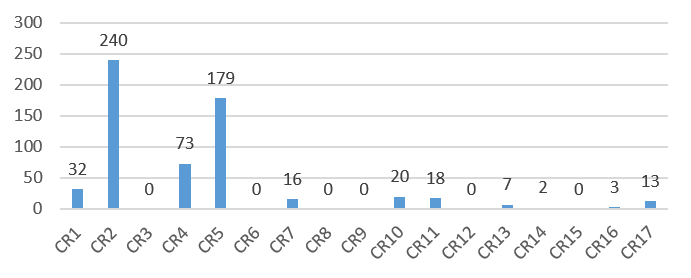
\includegraphics[width=0.9\textwidth]{./pics/chapter1pics/FrequencyICSE.png}
	%\vspace{-1em}
	\caption{Frequency of applied resolutions overall.}
	%\vspace{-1.5em}
	\label{fig:frequency_resolutions}
	\end{figure}
	
	
	\subsubsection{RQ2}
	
	%Our co-evolution approach is fully automatic and not guided by the developers, but rather by the matched patterns and their corresponding resolutions. Thus, \red{we can loose in correctness} in comparison to the  developers' manual co-evolution.
	To assess and measure the precision and recall of our automatic co-evolution, we first compared it with the manual co-evolution of the code that developers went through. 
	%To assess to what extent can our approach correctly co-evolve the code errors w.r.t. the manual co-evolution of the code that developers went through, we measured precision and recall.
	
	%Figure \ref{fig:correctness} 
	Table \ref{table:correctness} depicts the reached precision and recall of our automatic co-evolution approach for our nine case studies. We observe that the measured precision and recall varied, respectively from 48\% to 100\%, and from 51\% to 100\% reaching an average of, respectively 82\% precision and 81\% recall. 
	%
	%91,92+82,6+100+80,9+60,4+46,6+95,2+86,6+86,6 /9 = 81;20
	%91.92+82.6+100+80.9+60.4+46.6+95.2+86.6+86.6
	%
	%This means that our applied resolutions for the matched pattern usages for the code errors were correct w.r.t. the expected resolutions by the developers in \red{81\%}. 
	This shows the usefulness of the considered resolutions in Table \ref{table:ResolutionsCatalog} for the automatic co-evolution of the direct code errors in our case studies. %while meeting the developer's co-evolution needs. 
	
	\begin{table}[t]
	\caption{Measured precision and recall of our projects.}
	\label{table:correctness}
	\centering
	%
	%\small
	%\hspace*{-1em}
%	\resizebox{17.5cm}{!}{
		\begin{tabular}{
				@{\hskip3pt}l@{\hskip3pt}l@{\hskip3pt}l@{\hskip3pt}l@{\hskip3pt}l@{\hskip3pt}l@{\hskip3pt}l@{\hskip3pt}l@{\hskip3pt}l@{\hskip3pt}l@{\hskip3pt}}
			\toprule 
			Projects & P1 & P2 & P3 & P4 & P5 & P6 & P7 & P8 & P9 \\ \midrule%{2-10}
			precision & 90\%  & 80\%   & 100\%    & 81\%   & 58\%   & 48\%   & 98\%   & 93\%   & 93\% \\ \midrule
			recall & 66\%  & 83\%   & 100\%    & 75\%   & 58\%   & 51\%   & 94\%   & 100\%   & 100\% \\
			\bottomrule
		\end{tabular}
%	}
	\end{table}
	
	%\begin{figure}
	%	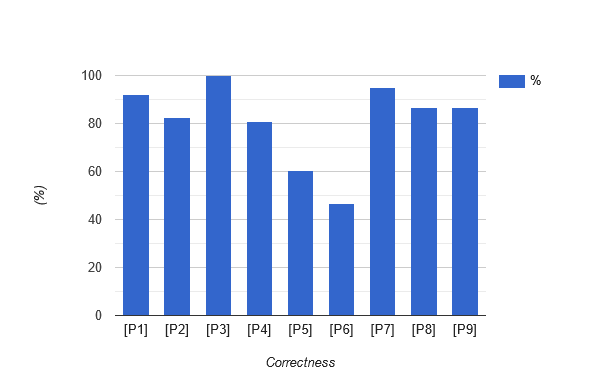
\includegraphics[width=0.6\textwidth]{pics/correctness.png}
	%\caption{Measured correctness of our projects.}
	%    \label{fig:correctness}
	%\end{figure}
	
	
	We further investigated the cause of lowering precision and recall, i.e., the cases where our automatic co-evolution did not match the expected resolutions. 
	The main observation is that several errors that could have been co-evolved by maintaining them were deleted by the developers in the manually evolved version of the code. Rather than to delete the erroneous code, our approach was able to successfully co-evolve and maintain it. 
	%
	For example, in the project \emph{P5}, we observed errors in the code due to moves of the properties \emph{maxUsedMemoryInBytes} and \emph{totalExecutionTimeInSeconds} and its rename to \emph{discoveryTimeInSeconds}. 
	%
	Our approach automatically co-evolved them and maintained the erroneous code, by renaming the setter and extending its path. Whereas, the developers' manual co-evolution consisted of deleting the impacted code. This may hint at a lack of automated co-evolution support that would have easily maintained the code in the new version rather than deleting it.  \red{Thus, our co-evolutions here are valid alternatives even if it did not match the correct manual co-evolution.}
	
	\begin{comment}
	
	\setulcolor{red}
	%,xleftmargin=0.2cm,,xrightmargin=-0cm,framexleftmargin=+6pt,frame=single
	\begin{lstlisting}[language=Java,breaklines=true,mathescape,literate={\-}{}{0\discretionary{-}{}{}},caption=Excerpt of the error in the code of the project P5.\label{lis:P5_V1}]
		//in the class Repport.java
		...
		discovery.(*\ul{setMaxUsedMemoryInBytes}*)(maxUsedMemory);
		discovery.(*\ul{setTotalExecutionTimeInSeconds}*)(...);
		...
	\end{lstlisting}
	
	\setulcolor{green}
	%,xleftmargin=0.2cm,,xrightmargin=-0cm,framexleftmargin=+6pt,frame=single
	\begin{lstlisting}[language=Java,breaklines=true,mathescape,literate={\-}{}{0\discretionary{-}{}{}},caption=Excerpt of the co-evolved error in the code of the project P5.\label{lis:P5_V2}]
		//in the class Report.java
		...
		discovery.(*\ul{getIterations().get(0).}*)  
		(*\ul{setMaxUsedMemoryInBytes}*)(maxUsedMemory);
		discovery.(*\ul{getIterations().get(0).}*) 
		(*\ul{getDiscoveryTimeInSeconds}*)(...);
		...
		
	\end{lstlisting}
	
	\end{comment}
	
	\red{It is worth noting that the order of the resolutions’ application is following the order of the treated metamodel changes. It may affect the number of iterations of Algorithm~\ref{algo :overallalgo} but it will neither affect the value of recall and precision nor the final result of the co-evolved code.}
	
	Finally, to check the behavioral effect of the co-evolution, we observed the tests' execution that we generated for the original and co-evolved code. %In total, respectively for the original and co-evolved versions. %, \red{xyz} and \red{xyz} test case were generated for the the nine projects, with \red{xyz} and \red{xyz} passing test, \red{xyz} and \red{xyz} failing tests, and \red{xyz} and \red{xyz} crashed tests due to an error. 
	Table \ref{table:test_results} depicts the test execution results. In \emph{[P1, P5, P6, P8, and P9]} similar tests were generated for the original and co-evolved versions. Whereas in \emph{[P2, P3, P7]} there were common tests as well as different generated tests, while we could also not generate tests for \emph{[P4]}. In most cases, we observe that the percentages of passing, failing, and erroneous tests were the same with no significant changes after the co-evolution. 
	Therefore, it suggests that our automatic co-evolution is behaviorally correct by not altering the code behavior of the original projects. 
	
	
	\begin{table*}[t]
	%\begin{wraptable*}{r}{5.5cm}
	\centering
	\caption{Observed test before and after co-evolution. [Legend: Before (V1) -- After (V2) ]}
	\label{table:test_results}
	%
	%\small
	%\hspace*{-2em}
	\resizebox{16cm}{!}{
		\begin{tabular}{
				@{\hskip3pt}c@{\hskip3pt}|c@{\hskip3pt}|c@{\hskip3pt}|c@{\hskip3pt}|c@{\hskip3pt}|c@{\hskip3pt}|c@{\hskip3pt}|c@{\hskip3pt}|c@{\hskip3pt}}
			\toprule 
			Projects & P1 & P2 & P3 & P5 & P6 & P7 & P8 & P9 \\ \midrule%{2-10}
			\begin{tabular}[c]{@{}l@{}}$N^{o}$ \\ tests\end{tabular} &  1987 -- 1987 & 2261 -- 2073  &  475 -- 555   & 67 -- 67  &  427 -- 427  &  142 -- 251  &  105 -- 105  &  75 -- 75 \\ \midrule
			\begin{tabular}[c]{@{}l@{}}$N^{o}$ \\ pass\end{tabular} & \begin{tabular}[c]{@{}l@{}} 826 -- 826 \\(41\% -- 41\%)\end{tabular} & \begin{tabular}[c]{@{}l@{}}  1221 -- 1161 \\ (54\% -- 56\%)\end{tabular} &\begin{tabular}[c]{@{}l@{}}  349 -- 417  \\ (73\% -- 75\%)\end{tabular}  & \begin{tabular}[c]{@{}l@{}}32 -- 32 \\ (47\% -- 47\%)\end{tabular}  &  \begin{tabular}[c]{@{}l@{}} 2 -- 2 \\(0.4\% -- 0.4\%)\end{tabular}    & \begin{tabular}[c]{@{}l@{}} 18 -- 103\\(12\% -- 41\%) \end{tabular}  &\begin{tabular}[c]{@{}l@{}}  16 -- 16\\(18\% -- 17\%) \end{tabular} & \begin{tabular}[c]{@{}l@{}} 14 -- 13 \\(15\% -- 15\%)\end{tabular}  \\ \midrule
			\begin{tabular}[c]{@{}l@{}}$N^{o}$\\ fail\end{tabular} &\begin{tabular}[c]{@{}l@{}} 14 -- 14\\ (0.7\%--0.7\%) \end{tabular}  & \begin{tabular}[c]{@{}l@{}} 36 -- 16 \\ (1,6\% -- 0,8\%)\end{tabular}  & \begin{tabular}[c]{@{}l@{}} 3 -- 3  \\(0.6\% -- 0,5\%)\end{tabular} & \begin{tabular}[c]{@{}l@{}}  2 -- 2  \\(2.9\% -- 2.9\%)\end{tabular} & \begin{tabular}[c]{@{}l@{}} 0 -- 0 \\(0\% -- 0\%)\end{tabular} & \begin{tabular}[c]{@{}l@{}}3 -- 4 \\(2.1\% -- 1.5\%)\end{tabular}  & \begin{tabular}[c]{@{}l@{}} 3 -- 3 \\(2.8\% -- 2.8\%)\end{tabular}  & \begin{tabular}[c]{@{}l@{}} 1 -- 1  \\(1.3\% -- 1.3\%)\end{tabular}\\ \midrule
			\begin{tabular}[c]{@{}l@{}}$N^{o}$\\ error\end{tabular} &\begin{tabular}[c]{@{}l@{}} 1147 -- 1147\\ (57\%--57\%) \end{tabular}&  \begin{tabular}[c]{@{}l@{}} 1004 -- 896 \\ (44\% -- 43\%)\end{tabular}  &  \begin{tabular}[c]{@{}l@{}}123 -- 135 \\(25.8\% -- 24.3\%)\end{tabular}  & \begin{tabular}[c]{@{}l@{}}33 -- 33\\(49.2\% -- 49.2\%)\end{tabular}  & \begin{tabular}[c]{@{}l@{}} 425 -- 425 \\(99.5\% -- 99.5\%)\end{tabular} &  \begin{tabular}[c]{@{}l@{}}121 -- 144 \\(85.2\% -- 57.3\%)\end{tabular} & \begin{tabular}[c]{@{}l@{}} 86 -- 86 \\(81.9\% -- 81.9\%)\end{tabular} & \begin{tabular}[c]{@{}l@{}} 60 -- 61\\(80\% -- 81.3\%)\end{tabular}\\ 
			\bottomrule
		\end{tabular}
	}
	%\end{wraptable*} 
	\end{table*}
	
	\begin{tcolorbox}[boxsep=-2pt]
	\textbf{$\boldsymbol{RQ_2}$ insights:}
	
	Our automatic co-evolution reached an average of an 82\% precision and 81\% recall.
	It was able to co-evolve and maintain erroneous code that developers unnecessarily deleted. 
	Generated tests for original and co-evolved code further showed that our co-evolution is not impacting the original code behavior w.r.t. the generated tests. 
	\end{tcolorbox}
	
	
	\begin{comment}
	
	
	\kaouter{ Discussion :1million
		1-The high-level intuition behind our approach is that
		we apply a targeted co-evolution by propagating the impacting metamodel changes only to the code errors directly, rather than browsing all code elements statically to fetch the possible impacts.
		Our automatic coevolution approach tries to mimic the developers' behavior with known resolutions when co-evolving the code errors in an “iterative way”. After the application of each resolution, the compilation unit is refreshed to get the list of the new compilation errors for the next iteration.
		
		2- the applied resolutions are related to the distribution of the impacting metamodel changes (see \ref{table:ResolutionsCatalog} ). However, there is no relation between the distribution of the applied resolution and the recall and precision that rather depends on “if” the automatic resolutions match "or not" the manual developer’s expected resolutions. Moreover, we did not randomly and synthetically choose the metamodel changes and their types in the evaluation. Rather, we took the realistic developers' evolutions of the metamodels in our selected real-world software projects.
		3- there are similarities with API migration approaches \cite{henkel2005catchup,andersen2010generic} on resolving errors in the client code, approaches do not handle all the equivalents of the impacting metamodel changes we do (\ref{table:ResolutionsCatalog}) and that occurred in our case studies. Therefore, we did not consider them as a baseline because we know apriori that too many changes would not be treated, hence, the comparison would be unfair and biased
		4-.Moreover, EMF is used for the implementation and evaluation, but our approach conceptually remains valid for other abstracted models that affect a Java code, such as in JHipster or OpenAPI.
		
	}
	
	
	%\DK{yes, i think this goes to discussion section 4.5}
	\subsection{Discussion}
	We now discuses our approach and the obtained results. 
	\end{comment}
	
	
	\subsubsection{RQ3}
	
	%\paragraph{Comparison with Quick Fixes}
	
	
	\begin{table*}[t]
	\centering
	\caption{Number of applied Quick Fixes for each project and per evolved metamodel.}
	\label{AppliedQF}
	\resizebox{16cm}{!} {
		\begin{tabular}{lllll}
			\toprule
			\begin{tabular}[c]{@{}l@{}}Evolved \\ metamodels\end{tabular} & \begin{tabular}[c]{@{}l@{}}Co-evolved \\ projects\end{tabular}  & \begin{tabular}[c]{@{}l@{}} \% of  \\eliminated \\ errors  \end{tabular} & \begin{tabular}[c]{@{}l@{}} $N^{o}$ of applied \\ Quick Fixes \end{tabular}  & Total
			\\ \midrule %& \begin{tabular}[c]{@{}l@{}} $N^{o}$ of \\applications \end{tabular}			
			
			\multirow{4}{*}{\begin{tabular}[c]{@{}l@{}}OCL \\ Pivot.ecore\end{tabular}} & $[P1]$ & 82\% 
			& \begin{tabular}[c]{@{}l@{}} 
				$  [$Create Class X$] $: 3, $ [$Create method m $] $: 27 , 
				\\  $[$Change m to m' $] $: 60,$[ $Add cast $] $: 59,
				\\  $[ $Change type (of variable or return type of method) $] $: 17,
				\\  $[ $Add unimplemented methods $] $: 43,
				\\ $[ $Create constants $] $: 15,  $[ $Remove argument $] $: 1.
			\end{tabular}  & 225\\ \cmidrule{2-5}			
			
			& $[P2]$ & 41\% 
			&\begin{tabular}[c]{@{}l@{}}
				$ [ $Create method $] $: 4,$[ $Change to m' $] $:11,\\
				$ [ $change type of var or return type $] $: 1,\\
				$ [ $Add unimplemented methods $] $: 2,
				
			\end{tabular}  & 18\\ \midrule			
			\multirow{6}{*}{\begin{tabular}[c]{@{}l@{}}Modisco \\ Benchmark.\\ecore\end{tabular}}  &  $[P3]$& 100\%
			& \begin{tabular}[c]{@{}l@{}}  
				%  $[ $  $] $
				$[ $ Create Class X  $] $: 6,  $[ $ Add unimplemented methods  $] $: 1
			\end{tabular}  & 7\\ \cmidrule{2-5}			
			
			& $[P4]$ &100\% 
			& \begin{tabular}[c]{@{}l@{}} 
				$[ $ Create Class X $] $: 2,$[ $  Create method $] $: 8,\\ $[ $ Change m to m' $] $; 5, $[ $ Remove argument $] $: 1,\\ $[ $ Add cast $] $ : 6
			\end{tabular}  & 22\\ \cmidrule{2-5}			
			
			& $[P5]$ &83\%
			& \begin{tabular}[c]{@{}l@{}}
				$[ $  Create Method $] $: 17,  $[ $ Change method m to m' $] $: 16, \\ $[ $ Remove argument $] $: 2,  $[ $ Change type of var or return type $] $: 1,\\  $[ $ Add Cast$] $: 16.
				
			\end{tabular}& 52  \\ \cmidrule{2-5}			
			
			& $[P6]$&67\% 
			& \begin{tabular}[c]{@{}l@{}}
				$[ $ Change method m to m' $] $: 4, $[ $ Add unimplemented methods  $] $: 2,\\ $[ $ Create Constant$] $:9, $[ $ change type $] $ : 2,\\$[ $ Add Cast  $] $: 6
				
			\end{tabular}& 23  \\ \midrule			
			
			\multirow{4}{*}{\begin{tabular}[c]{@{}l@{}}Papyrus \\ ExtendedTypes.\\ecore\end{tabular}} &  $[P7]$&69\%
			& \begin{tabular}[c]{@{}l@{}} 
				$[ $ Create Class X $] $: 3,  $[ $ Create method m $] $: 9,\\  $[ $ Change method m to m' $] $: 13,  $[ $Change type of var or return type  $] $: 5, \\$[ $ Add Cast $] $: 4,  $[ $Add unimplemented methods$] $: 2.
				
			\end{tabular} & 36 \\ \cmidrule{2-5}			
			
			&  $[P8]$ &93\%
			& \begin{tabular}[c]{@{}l@{}}
				$[ $ Create Class X $] $: 1,  $[ $ Create method $] $ : 14,\\ $[ $ Create Const $] $ :3,  $[ $ Add Cast$] $: 2,\\  $[ $ Change method m to m' $] $:3.
			\end{tabular} & 23 \\ \cmidrule{2-5}			
			
			&  $[P9]$ &93\% &
			
			\begin{tabular}[c]{@{}l@{}}
				$[ $ Create Class X $] $: 1,  $[ $ Create method $] $ : 14,\\ $[ $ Create Constant $] $ :3,  $[ $ Add Cast$] $: 2,\\  $[ $ Change method m to m' $] $:3.
			\end{tabular} & 23 \\ \midrule			
			Total &&&& 429 \\ \bottomrule
			
			
			%	& CS14:MPRPS                                                                                                           & \begin{tabular}[c]{@{}l@{}} $\rhd [R4]$ \\ $\rhd [R6]$ \\ $\rhd [R9]$ \end{tabular} &   \begin{tabular}[c]{@{}c@{}} 4 \\ 3 \\ 4 \end{tabular}     \\ 			
		\end{tabular}  
		
	}
	%\vspace{-0.5em}
	\end{table*}
	
	The first baseline we compare to is the quick fixes available in the IDE since they are widely used by developers to repair code errors%yu2012maintaining QF are used by developers usually to resolve compiling errors.
	%
	~\cite{10.1145/2384616.2384665}, and more importantly, they have not been compared to code co-evolution approaches before. 
	To compare with the quick fixes as a baseline, we implemented the automatic application of quick fixes as an option in our plugin. It is a variant of our Algorithm \ref{algo :overallalgo} that only applies the quick fixes on the errors. 
	The algorithm browses the errors of each compilation unit and applies the first proposed quick fix, since by default Eclipse IDE\footnote{See \emph{org.eclipse.jdt.ui.text.java.CompletionProposalComparator}} order the quick fixes by \emph{relevance}. Note that all executions herein terminated normally without any infinite loop.
	%The selection of the first quick in the list of proposals is due to the strategy of proposals ordering of eclipse. \texttt{CompletionProposalComparator} of eclipse proposes two criteria: by relevance and alphabetic order. Eclipse default settings opt for ordering by relevance.
	
	%It stops in two cases: 1) when only errors without any quick fix proposal remain, or 2) when the application of a quick fix causes an infinite loop \cite{cuadrado2018quick,khelladi2019detecting}, i.e., a cycle of applying a quick fix that causes a previously fixed error (A $\mapsto$ B $\mapsto$ A $\mapsto$ B $\mapsto$ ...).   
	%(Error A quick fixed, error B appears \textless--\textgreater 
	% Error B quick fixed, error A appears), infinite side-effect cycle. 
	
	
	
	In Table~\ref{AppliedQF}, we present the percentage of errors that quick fixes eliminated for each project, and the frequencies of each type of applied quick fixes. 
	%we give the number of quick fixes applied per type, 
	%\red{to help us to analyse the quick fixes' reaction to the different types of changes.}\todo{what ?} 
	
	While the quick fixes eliminated from 41\% to 100\% errors, we found that the precision and recall of automatic quick fixes are equal to 0, because no correction was applied as expected to the manual developers' resolutions. That is why we refer to the errors are eliminated by the quick fixes and not corrected or co-evolved. 
	For example, concerning errors caused by class or property deletion from the metamodel, renaming a class or an attribute, moving, pushing, or pulling attributes or methods from a class to another, the quick fixes proposed to create them back in their old containers. This is in contradiction of the applied metamodel changes.  
	%for some errors, the usage of the metamodel class in the code is super %interface, and when applying the first quick fix, it will create a class %and not an interface
	%duplicate case
	For errors caused by changing a variable's type, the quick fixes always suggested adding a cast with a wrong type. 
	
	%Adding a declaration or an implementation of missing or renamed method causes a major problem of polymorphism on which metamodeling is based on. In the case of adding a method declaration in an interface, all classes that implement this interface will ask to "add unimplemented method", and by applying this quick fix, an empty methods will be added. These corrections do not meet the specifications of the metamodel changes. 
	
	Unlike our approach, quick fixes do not take in consideration the context of the impacted code and the information contained in its causing metamodel changes. For example, the quick fix \texttt{create the missing method \emph{m()}} is applied no matter the metamodel change (i.e., deletion, moving, pulling, or pushing changes) or the impacted code location (i.e., statement, variable declaration, parameter, etc.). %this invocation is located in a complex statement, in a variable declaration, or in any other position in the code AST. 
	Our approach takes into account the context of the impacted code and the causing change thanks to the use of pattern matching (see Section~\ref{pattern_matching}). 
	% either the pattern MoveProperty\_UpperBoundSingle or the pattern MoveProperty Upper\_BoundMultiple is detected then
	
	
	For instance, after a move property change, the resolution $[CR7]$ or $[CR8]$ is applied, respectively. Thus, taking into consideration the embedded information in the causing metamodel change, namely the origin class, the target class, and the multiplicity of the reference between them.
	
	
	
	\begin{tcolorbox}[boxsep=-2pt]
	\textbf{$\boldsymbol{RQ_3}$ insights:}
	The automatic application of quick fixes leads to a faulty evolved code. The same type of quick fixes is applied regardless of the context of the impacted code. With 0 precision and recall, we can conclude the inability of Eclipse quick fixes to co-evolve correctly the code with the evolution of the metamodel. 
	\red{}
	
	\end{tcolorbox}
	
	
	
	\subsubsection{RQ4}
	%\paragraph{Comparison with State of the art co-evolution}
	
	%%%%%%%%%%%%%%%%%%%%Comparaison with prior work %%%%%%%%%%%%%%%%%%%%%%%%%%%%%%%%%%%%%%%%%%%%%%%%%%%%%%%%%
	%%%%%Table recall and precision per project %%%%
	\begin{table*}[t]
	%\begin{wraptable*}{r}{5.5cm}
	\centering
	\caption{Comparison between our automatic co-evolution approach and the semi-automatic co-evolution approach. [Legend: Precision(P) -- Recall(R) ]}
	\label{table:comparison_AC_vs_SC}
	%
	\normalsize
	%\hspace*{-2em}
	\resizebox{17cm}{!}{
		\begin{tabular}{
				@{\hskip3pt}c@{\hskip3pt}|c@{\hskip3pt}|c@{\hskip3pt}|c@{\hskip3pt}|c@{\hskip3pt}|c@{\hskip3pt}|c@{\hskip3pt}|c@{\hskip3pt}|c@{\hskip3pt}|c@{\hskip3pt}|c@{\hskip3pt}}
			\toprule 
			Projects & P1 & P2 & P3& P4 & P5 & P6 & P7 & P8 & P9& Total \\ \midrule%{2-10}
			\begin{tabular}[c]{@{}l@{}} Our automatic approach\end{tabular} & \begin{tabular}[c]{@{}l@{}} 90\%(P)\\ 66\%(R)\end{tabular} & \begin{tabular}[c]{@{}l@{}} 80\%(P)\\ 83\%(R)\end{tabular} &  \begin{tabular}[c]{@{}l@{}} 100\%(P) \\ 100\%(R) \end{tabular} & \begin{tabular}[c]{@{}l@{}}81\%(P) \\ 75\%(R)\end{tabular} & \begin{tabular}[c]{@{}l@{}} 58\%(P) \\ 58\%(R)\end{tabular} & \begin{tabular}[c]{@{}l@{}} 48\%(P) \\ 51\%(R)\end{tabular} & \begin{tabular}[c]{@{}l@{}} 98\%(P) \\ 94\%(R)\end{tabular} & \begin{tabular}[c]{@{}l@{}}  93\%(P) \\ 100\%(R)\end{tabular} & \begin{tabular}[c]{@{}l@{}} 93\%(P) \\ 100\%(R)\end{tabular}
			& \begin{tabular}[c]{@{}l@{}} 82\%(P) \\ 81\%(R)\end{tabular}
			\\ \midrule
			
			\begin{tabular}[c]{@{}l@{}} \textbf{Semi-automatic approach \cite{Khelladi2020}}\end{tabular} & \begin{tabular}[c]{@{}l@{}}92\%(P) \\ 92\%(R)\end{tabular} & \begin{tabular}[c]{@{}l@{}} 93\%(P) \\ 86\%(R)\end{tabular} &\begin{tabular}[c]{@{}l@{}} 100\%(P) \\ 100\%\end{tabular}  & \begin{tabular}[c]{@{}l@{}}100\%(P) \\ 100\%(R) \end{tabular}  &  \begin{tabular}[c]{@{}l@{}}100\%(P) \\ 100\%(R)\end{tabular}    & \begin{tabular}[c]{@{}l@{}} 48\%(P) \\ 48\%(R)\end{tabular}  &\begin{tabular}[c]{@{}l@{}} 100\%(P) \\ 100\%(R)\end{tabular} & \begin{tabular}[c]{@{}l@{}}100\%(P) \\ 100\%(R)\end{tabular} & \begin{tabular}[c]{@{}l@{}}100\%(P) \\ 100\%(R)\end{tabular}   & \begin{tabular}[c]{@{}l@{}}92\%(P) \\ 91\%(R)\end{tabular}  \\
			\bottomrule
			
		\end{tabular}
	}
	
	%\end{wraptable*} 
	\end{table*}
	
	%%%% Text about comparison AC vs SC
	% we treat more changes. the impact analysis is not the same.
	
	
	
	We now compare our approach to the state of the art of metamodel and code co-evolution, namely our previous work \cite{Khelladi2020}. It runs an impact analysis to trace the impacts in the code, while we rely on the compilation errors after regenerating the code API from the evolved metamodel. 
	We also consider an additional change of Pull property and add a new resolution for it ($CR14$). 
	We further distinguish with our previous work by checking behavioral correctness with tests (before/after co-evolution) and by comparing to two baselines. 
	Yet, the main difference is it being semi-automatic requiring intervention to decide between alternative resolutions to co-evolve the code, while we fully automate this decision based on our pattern matching process. Thus, intuitively, it will likely perform better than a fully automatic co-evolution. RQ4 aims to measure this difference.  
	
	%The semi-automatic approach of code co-evolution of Khelladi et al. \cite{Khelladi2020} starts by change detection and an impact analysis. This approach takes into account the types of changes listed in Table \ref{mmchanges}, except for the "Pull property" change type. While the impacted parts in code, in our approach, consist of compiling errors, Khelladi et al. \cite{Khelladi2020} proceed by a static analysis without compilation. Each evolved metamodel is traced through the AST of the generated code elements and their usages in the AST of the additional code. The impacted nodes are then coevolved using the catalog of resolutions \ref{table:ResolutionsCatalog} ( that does not include $CR14$). 
	%Our approach is 100\% automatic thanks to the pattern matching process \ref{pattern_matching}. In the case of an impact that supports more than one resolution, Khelladi et al. give the developer the choice to select one of the possible resolutions.
	%This semi-automatic approach is evaluated on the nine projects described in Table \ref{CaseStudies_CoEvolution}. Unlike our evaluation, Khelladi et al. used only precision and recall metrics in their evaluation process, without any other checking of the behavioral correctness of their semi-automatic co-evolution approach. 
	Table \ref{table:comparison_AC_vs_SC} shows precision and recall values of our approach and the semi-automatic co-evolution approach~\cite{Khelladi2020}. 
	We notice that the semi-automatic co-evolution approach~\cite{Khelladi2020} outperforms our automatic co-evolution approach by a small margin in terms of precision and recall. % ( 92\% over 82\%) and recall(91\% over 81\%). However, the margin between the values remains small. 
	On average, we had 82\% precision and 81\% recall in full automatic co-evolution compared to 92\% precision and 91\% recall in semi-automatic co-evolution. 
	This is due to the fact that our approach favors the least deletion when possible $[CR1]$ over $[CR3]$, or $[CR4]$ over $[CR2]$, while the semi-automatic approach favors integral deletions $[CR3]$ over $[CR1]$, or $[CR2]$ over $[CR4]$. %, and this integral deletion matches the developers' co-evolved version.
	Overall, we observe that the trade-off between full and semi-automatic co-evolution leads to only a reduction of -10\% in precision and recall while still maintaining them at a high level ($>$ 81\%). This small reduction in performance provides a bigger benefit of speeding up the co-evolution and removing the burden of manual intervention from developers on every code error. Indeed, rather than spending time in guiding the co-evolution at every error, developers can automatically perform it in couples of minutes, in particular, if thousands of errors must be co-evolved after metamodel evolution.
	
	
	\begin{tcolorbox}[boxsep=-2pt]
	\textbf{$\boldsymbol{RQ_4}$ insights:}
	Fully automating metamodel and code co-evolution performs less than a semi-automatic co-evolution, but still gives a high precision and recall of ($>$ 81\%) while removing the burden of manual intervention from developers on every code error to co-evolve. 
	\end{tcolorbox}
	
	% Tests for correctness checking
	% Precision, Recall
	%%%%%%%%%%%%%%%%%%%%%%%%%%%%%%%%%%%%%%
	
	% describe the approach
	\subsection{Discussion and limitations}
	This section discusses the approach and the observed results. 
	
	The high-level intuition behind our approach is that we apply a targeted co-evolution by propagating the impacting metamodel changes only to the code errors directly, rather than browsing all code elements statically to fetch the possible impacts.
	Our automatic co-evolution approach tries to mimic the developers' behavior with known resolutions when co-evolving the code errors in an “iterative way”. After the application of each resolution, the list of errors %compilation unit 
	is refreshed to get the list of the new compilation errors for the next iteration.
	% relation betsween the input and the output of the evaluation
	
	Moreover, Table \ref{AppliedResolutions} shows the distribution of applied resolutions. It is related to the distribution of the impacting metamodel changes (see Table~\ref{table:ResolutionsCatalog}) since for a given impacting change, a specific set of resolutions can be applied. 
	However, there is no relation between the distribution of the applied resolution and the recall and precision, which depends more on 'if' the automatic resolutions match "or not" the manual developer’s expected resolutions. Moreover, we did not randomly and synthetically choose metamodel changes and their types in the evaluation. Rather, we took the realistic developers' evolutions of the metamodels in our selected real-world software projects. Thus, we did not influence the applied resolutions, which correspond only to the metamodel changes. Of course, having a different distribution of metamodel changes would result in a different distribution of applied resolutions. 
	
	Finally, we handled the evolution of one metamodel at once to co-evolve its impacts. Handling multiple metamodels is an interesting case, but is out-of-scope in this dissertation. Nonetheless, the first favorable scenario we can currently handle is to treat the multiple metamodels in sequence when they are independent of each other. The main limitation is in a second scenario where there are dependencies between the multiple metamodels. For example, a change "set type to T" in a metamodel A referencing a change "add T" in a metamodel B. Herein, the solution would be to find the order of metamodels in which to handle the co-evolution in sequence. This is left as future work. 
	
	\section{Threats to Validity}\label{ch1_threat}
	\noindent This section discusses threats to validity \cite{wohlin2012experimentation}.
	
	\subsection{Internal Validity.} To provoke the code errors, we had to replace the original metamodel evolution and to regenerate the code API. To reduce any bias in the source of errors, we decided to evolve one metamodel at a time. This increases the confidence in the source of the errors, and hence, their co-evolution. Dealing with conflicting errors that can mask each other due to the simultaneous evolution of several metamodels is left for future work.  
	Moreover, to measure the correctness, we analyzed the developers' manual co-evolution.
	To reduce the risk of misidentifying an expected resolution, for each impacted part of the code, we investigated the entire co-evolved class. If we did not find it, we further searched in other classes in case the original impacted part of the code was moved into another class. Thus, our objective was to reduce the risk of missing any correspondence between an error in the original code and its evolved version. Moreover, as our co-evolution relies on the quality of detected metamodel changes, we analyzed each detected change and checked whether it occurred between the original and evolved metamodels. This alleviates the risk of relying on an incorrect metamodel change that would degrade the pattern matching. 
	Note that the order of changes taken as input does not influence our co-evolution, but the order of errors we treat may affect the distribution of the applied resolutions. However, we took the order in which the errors were detected. 
	Finally, besides the manual checking of the co-evolved code, we used Evosuite as a test suites generation tool that has shown its efficiency in
	test generation as a state-of-the-art tool~\cite{DANGLOT2019110398,https://doi.org/10.1002/stvr.1601}. The main reason is that our projects did not have manually written tests. However, automatic test
	generation can even be more advantageous herein. Indeed, it generates tests for all
	public methods, whereas developers tend to manually write few tests for only some targeted methods. Thus, if relying only on manually written tests, there is a high risk of not assessing the behavioral correctness of many cases of code co-evolutions that are not covered by test cases. Despite the fact that generated tests can be better for our approach and its results allow us to measure the behavioral correctness of the co-evolution, %it is still not sufficient as it cannot replace the manual written tests. Further studies are needed here}.
it still can be combined with manual written tests.


\subsection{External Validity.} We implemented and evaluated our approach for EMF and Ecore metamodels and Java code. %As EMF metamodels rely on MOF \cite{MOF241} and object-oriented elements that can 
%Other object-oriented languages use different syntax but conceptually use the same constructions as in Java, such as C\# or C++.
Although co-evolution could theoretically be applicable for other languages, such as C\# or C++, we cannot generalize our results. Further experimentation on other languages is necessary. However, the only requirement to apply our approach to other languages is to parse the ASTs of the erroneous code and to adapt our resolutions to the new ASTs' structure.  

Furthermore, the evaluation was carried out on Eclipse projects in three languages. Thus, we cannot generalize our findings to other software languages and their implementations. However, our approach could be used to co-evolve Java code added on top of a generated code from a domain model, \eg from a UML class diagram or an entity model. %, such as JHipster that generates a complete and modern Web app or microservice architecture based on a domain model and a set of architectural choices. 
Nonetheless, more evaluations are still necessary. %\footnote{https://www.jhipster.tech/}

\subsection{Conclusion Validity.} Our evaluation showed promising results with an automatic code co-evolution that is fast and useful, with an average of~82\% precision and~81\% recall varying from~48\% to~100\%. The results also showed the usefulness of our approach and the resolutions proposed in our catalog in Table \ref{table:ResolutionsCatalog}. However, even though we evaluated it on nine projects with complex metamodel evolution, we plan to further evaluate on more case studies to have more insights and statistical evidence.  %further evaluation is needed on more case studies.
\begin{comment}
	
\end{comment}


\section{Conclusion}\label{ch1_conclusion}

In this chapter, we presented an approach to automatically co-evolve code when metamodels evolve. It relies on a pattern matching algorithm to match the different pattern usages of the metamodel generated code elements in the additional erroneous code. Once a direct error in the code is matched with a pattern usage, we can co-evolve it with its corresponding resolution. 
For indirect errors that cannot be matched, we apply the available quick fix to repair them. 
%
Our code co-evolution was evaluated on nine projects and three metamodels from three Eclipse EMF implementations. After re-generating the code API from the evolved version of the metamodel, hence, causing~837 errors in the additional code.
For the~771 direct errors, our automatic co-evolution approach was able to match 631 pattern usages and to apply~631 resolutions. It showed to be efficient and useful in co-evolving all direct errors in the code with an average of~82\% precision and~81\% recall varying from~48\% to~100\%. All~66 indirect errors were resolved by calling~5 quick fixes. Moreover, we checked the behavioral correctness of our approach by using test suites before and after code co-evolution. We observed that the percentage of passing, failing, and erroneous tests remained stable with insignificant variations in some projects. Thus, suggesting the behavioral correctness of the co-evolution. Finally, we found that the quick fixes are not able to correctly co-evolve the code. This is because they cannot exploit the context of the impacted code and relate it to the changes of the metamodel. 
\red{We also found that fully automating metamodel and code co-evolution performs less than a semi-automatic co- evolution, but still gives a high precision and recall of ($>$ 81\%) while removing the burden of manual intervention from developers on every code error to co-evolve.}


In summary, our work presents the following contributions :
1/ A fully automatic code co-evolution approach due to Ecore metamodel evolution based on pattern matching. 
2/ A prototype implementation of an Eclipse plugin to show the efficiency of our approach. % available publicly\footnote{\url{https://figshare.com/s/8986914e924300be77da}}.
3/ An evaluation based on four actions: 1) Measuring the co-evolution correctness. 2) Verifying the behavioral correctness using unit tests running before and after automatic code co-evolution. 3) Comparison with the state-of-the art semi-automatic co-evolution approach~\cite{Khelladi2020}. 4) Comparison with Quick Fixes popular tool.



%As future work, we first plan to explore ordering the errors in the code before co-evolving them. In fact, we co-evolve the errors in the same order they are retrieved by the JDT. Thus, we will investigate whether it could reach better correctness with faster co-evolution or not. 
%
%Finally, we plan to extend our resolutions with a replace resolution, based on distance metrics to find element replacements to co-evolve the code. \red{After that, we can rely on our approach to extend it with a search-based heuristics, such as genetic algorithms to explore different paths of co-evolution, in contrast to a single path that we compute in this paper. In particular, to explore the different alternative resolutions of $CR1-CR4$.}  

%
%a\kaouter{}
%\DK{either we put it as future work, maybe even in discussion above 4.5, and then refer to it here and say future work.}
%
%Finally, we will evaluate our approach on more case studies and on the case of simultaneous multiple metamodel evolution. 
%\section*{Acknowledgments.} The research leading to these results has received funding from the \emph{RENNES METROPOLE} under grant \emph{AIS no. 19C0330} and from \emph{ANR} agency under grant \emph{ANR JCJC MC-EVO$^{2}$ 204687}.

%\newpage
